\renewcommand{\thechapter}{\Roman{chapter}}
\chapter{Result and Discussion}
\renewcommand{\thechapter}{\arabic{chapter}}
\label{ch:Result and Discussion}
\thispagestyle{empty}

The results of the system development outlined in the previous chapter were presented and discussed in this chapter. After evaluating the specification of each system and undergo different design revision and integration, the study successfully identified and finalized the necessary components, tools and materials for each system.

\section{Developed 3D Point Cloud Scanner System (3D-PCSS)}

\subsection{3D-PCSS CAD Design Setup}

The 3D Point Cloud Scanner System hardware setup, as shown in Figure \ref{ch4:fig:cad_storage_bin}, consists of a 2D LiDAR Device fixed to a platform connected to a servo motor. This servo motor allows the platform to rotate, giving the LiDAR device an extra axis of movement. Inside the compartment is where the single-board computer along with other circuit components located. The detailed specification of each of the components is presented in appendix \ref{appen:a}.

\begin{figure}[H]
	\centering
	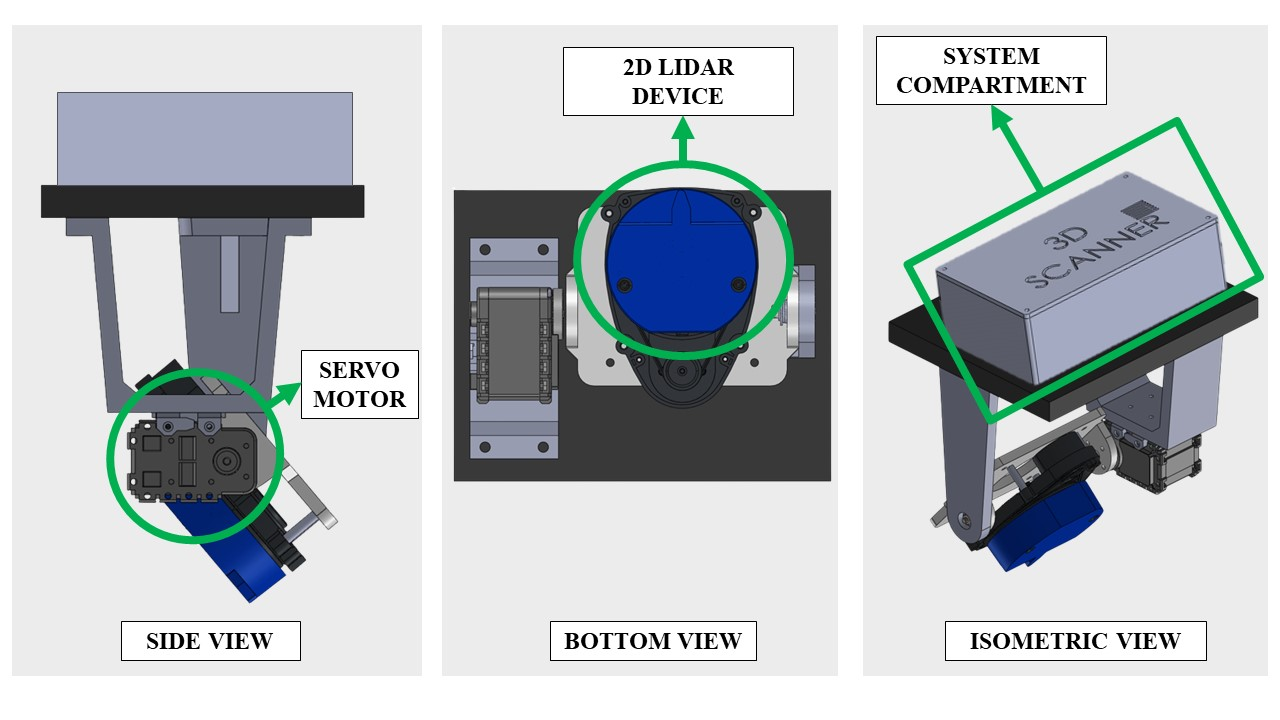
\includegraphics[width=1\textwidth]{Figures/3d-pcss-cad-design}
	\caption{Different View of the CAD Model Design of 3D-PCSS}
	\label{ch4:fig:cad_storage_bin}
\end{figure}

\subsection{Actual Design of the 3D-PCSS}

The actual development of the 3D-PCSS shown in figure \ref{ch4:fig:actual-3d-pcss} was constructed in accordance with the 3D CAD model design and the system is powered by a battery. Before the integration of the system, individual component testing were conducted to test and verify if such components function properly. The base platform, to which the 2D LiDAR device and servo motor are attached, was fabricated using aluminum metal. The system compartment is fabricated using a 3D printer and employing ABS material. Inside the compartment, the specific components and its category is shown in figure \ref{ch4:fig:specific-components}
\begin{figure}[H]
	\centering
	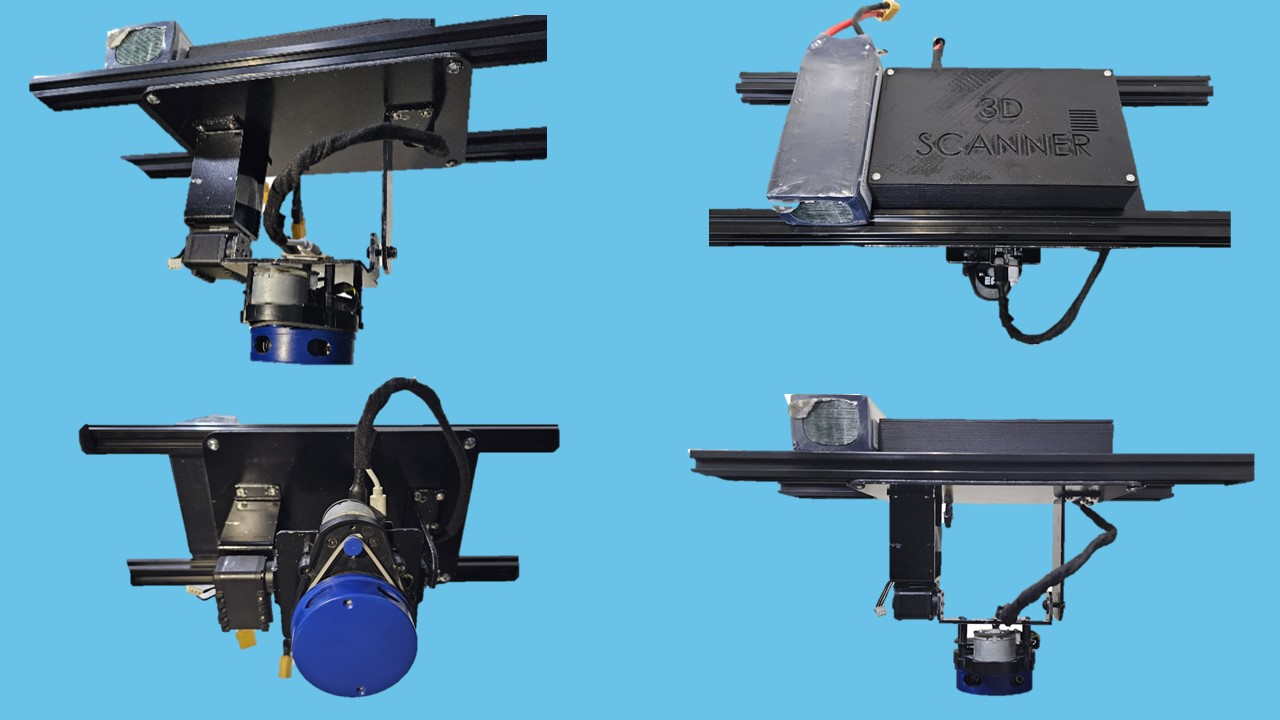
\includegraphics[width=1\textwidth]{Figures/actual-3d-pcss}
	\caption{Actual 3D-PCSS Developed}
	\label{ch4:fig:actual-3d-pcss}
\end{figure}

\begin{figure}[H]
	\centering
	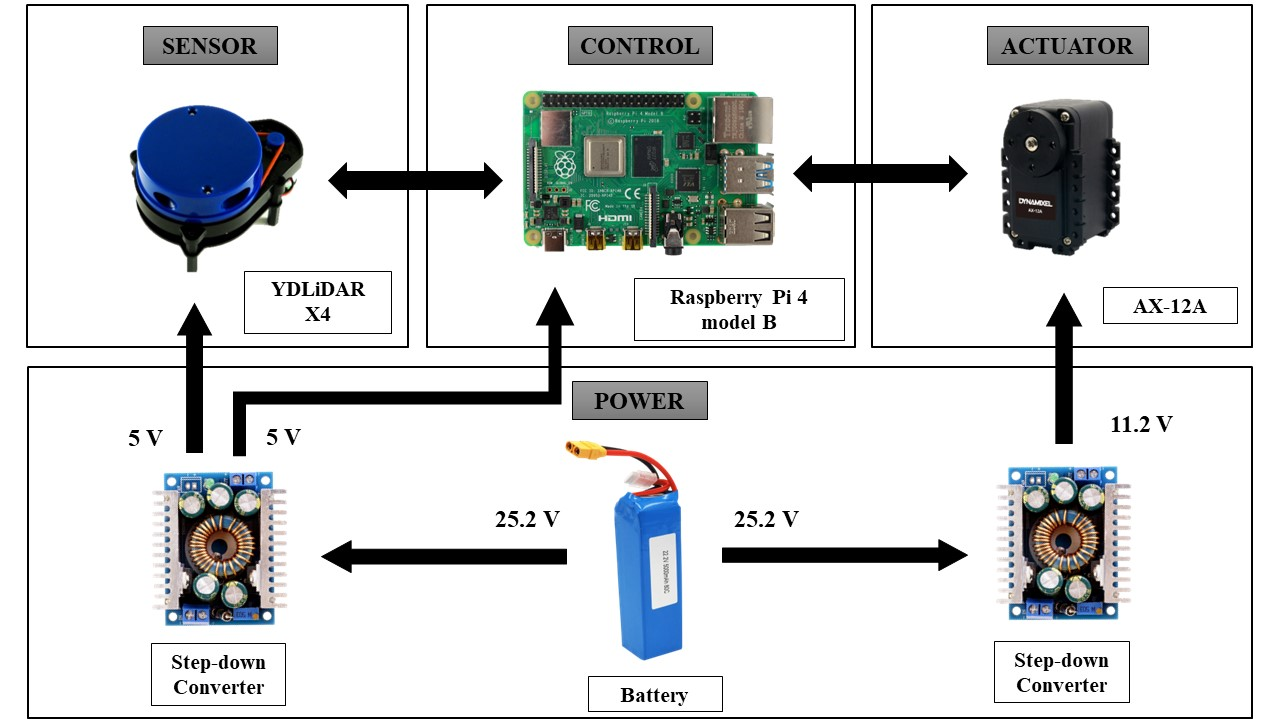
\includegraphics[width=1\textwidth]{Figures/specific-components}
	\caption{Specific Components of the System}
	\label{ch4:fig:specific-components}
\end{figure}

\section{Software Implementation}

The processes discussed in the previous chapter were implemented on the single-board computer (Raspberry Pi), playing a crucial role in the overall functionality of the 3D-PCSS. Figure \ref{ch4:fig:nodes-topics-relationships} illustrates the various nodes, topics, and their relationships in a publish-subscribe model. This implementation were apply after construction of the actual design of the 3D-PCSS. The arrows in the diagram show how data flows between the different nodes and its relationship to a corresponding topics. The ROS bridge server Node facilitates communication by relaying commands between the web application and the ROS framework via the ``/rosapi" service. Commands to start and stop scanning from the web interface are processed using the Remote Command Node within the system. The LiDAR Node captures data and publishes it as range values, while the Dynamixel Node and LiDAR Node synchronize their operations through the ``/dxl\_pos" topic. The Scan to 3D Point Cloud Mapping Node converts raw scan data into usable 3D point cloud data. Finally, the post-processing stage refines the point cloud data for volume measurement.

\begin{figure}[H]
	\centering
	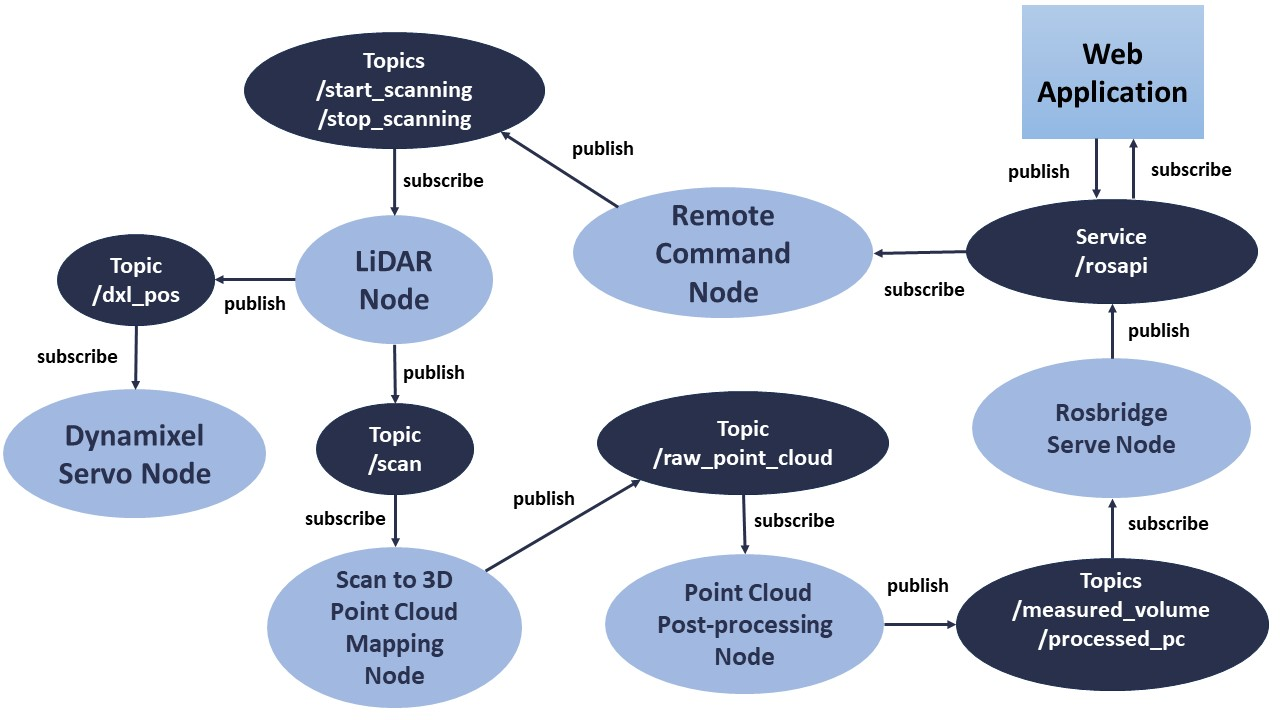
\includegraphics[width=1\textwidth]{Figures/nodes-topics-relationship}
	\caption{Nodes, Topics and their Relationships}
	\label{ch4:fig:nodes-topics-relationships}
\end{figure}

\section{Web-based User Interface Implementation}
A variety set of tools and frameworks were employed to enhance the functionality of the Web Interface. Table \ref{ch3:tab:tools-frameworks} outlines the various tools, frameworks, and libraries utilized in the implementation of the web-based user interface.

\begin{table}[H]
	\centering
	\caption{Tools and Frameworks Used in the Web-based User Interface}
	\label{ch3:tab:tools-frameworks}
	\begin{tabular}{|l|p{9cm}|}
		\hline
		\textbf{Tool/Framework} & \textbf{Description/Functionality}                                                                                                                                                \\ \hline
		jQuery                  & Used for simplifying JavaScript programming and DOM manipulation, jQuery is included via CDN for easy integration.                                                                \\ \hline
		Three.js                & This JavaScript library is utilized for rendering 3D graphics in a web browser. It enables the display of the 3D point cloud viewer within the application.                       \\ \hline
		EventEmitter2           & EventEmitter2 is employed for implementing event-driven programming, allowing efficient communication between different components of the application.                            \\ \hline
		roslib.js               & roslib.js is utilized for connecting the web application to the Robot Operating System (ROS), enabling communication with ROS nodes and topics.                                   \\ \hline
		Bootstrap               & The Bootstrap framework is employed for responsive design and styling of the user interface components. It ensures consistency and enhances the visual appeal of the application. \\ \hline
		Chart.js                & This JavaScript library is used for creating interactive charts and graphs to visualize data. It enhances the user experience by providing intuitive data representation.         \\ \hline
		ros3d.js                & ros3d.js is utilized for integrating ROS visualization capabilities into the web application. It facilitates the display of ROS topics such as point clouds and robot models.     \\ \hline
	\end{tabular}
\end{table}


These tools and frameworks collectively contribute to the functionality of the web-based user interface for the 3D-PCSS.

\subsection{UI Different Dashboard}
\subsubsection*{Main Dashboard Section}
The main dashboard of the UI, as shown in Figure X, consists of three distinct sections. On the left side, the System Status section provides visual feedback regarding the establishment of the connection with the system, allowing users to monitor and verify the connection status. Additionally, users can access a list of currently active topics by clicking the List of Topics button. In the center section, users can visualize and interact with the 3D point cloud data. This includes functionalities such as zooming in and out, moving the visualization, and conducting analysis. Moreover, in this section the start and stop scanning button is located, enabling users to control the scanning process directly from the dashboard. Finally, on the right side, users can find volume measurement values and other pertinent information, such as storage capacity values. The save button is also located in this section to store the empty space volume, Product volume and the percentage capacity of the storage bin in the database

\begin{figure}[H]
	\centering
	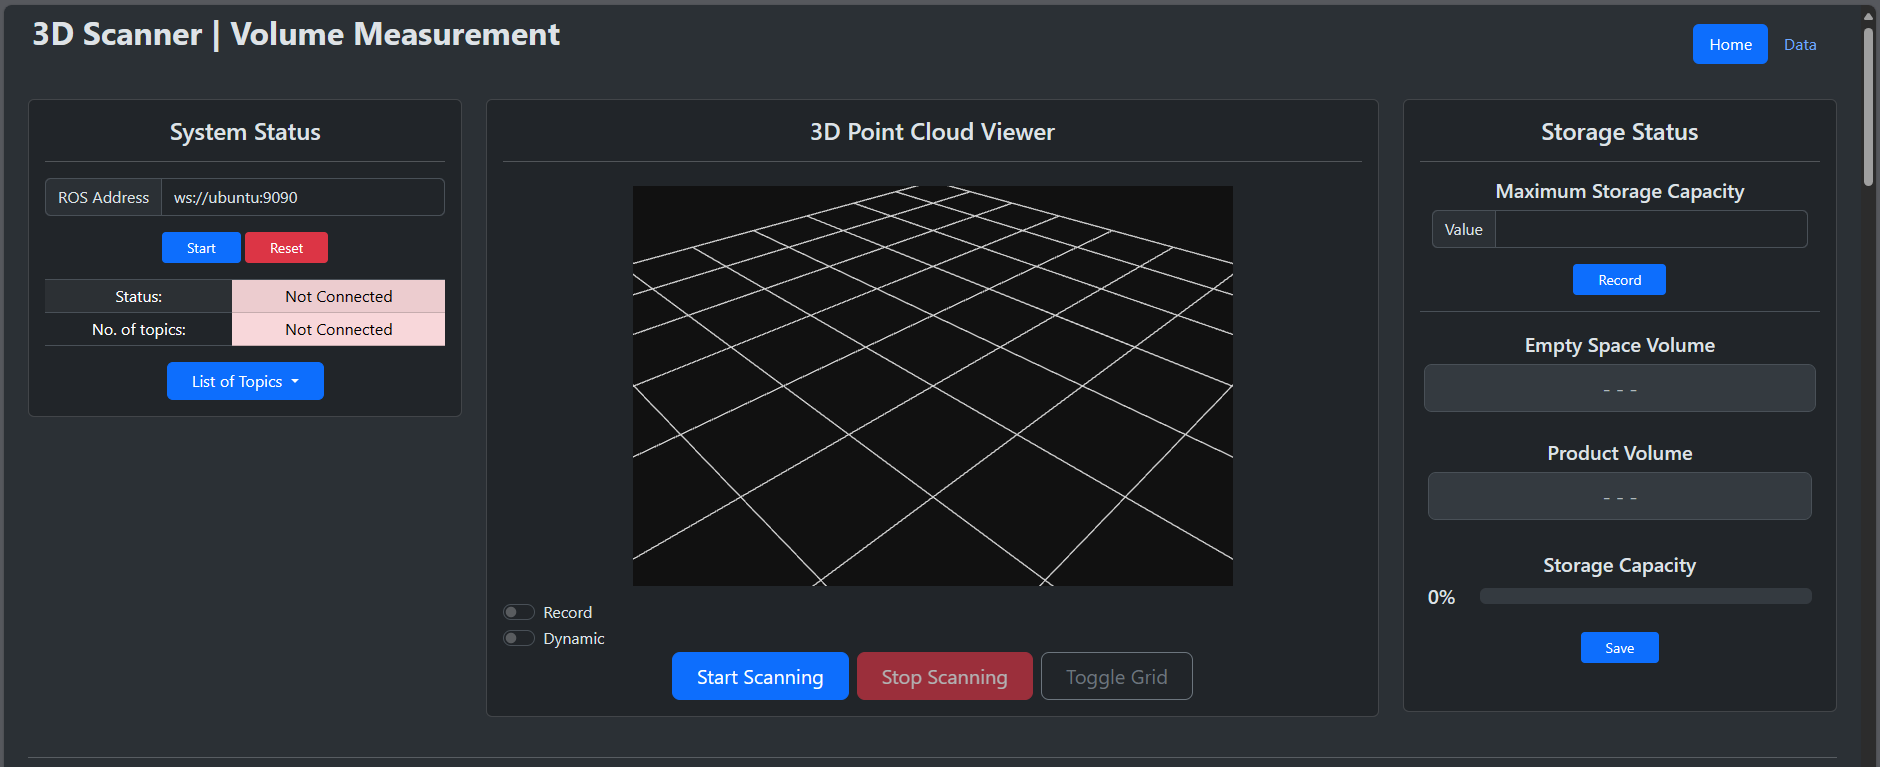
\includegraphics[width=0.9\textwidth]{Figures/main-dashboard}
	\caption{Main Dashboard of Web Interface}
	\label{ch4:fig:main-dashboard}
\end{figure}

\subsubsection*{Data Section}

In the data section of the dashboard, users can visualize both the data table and the graph, as depicted in Figures X and Y, respectively.

\begin{figure}[H]
	\centering
	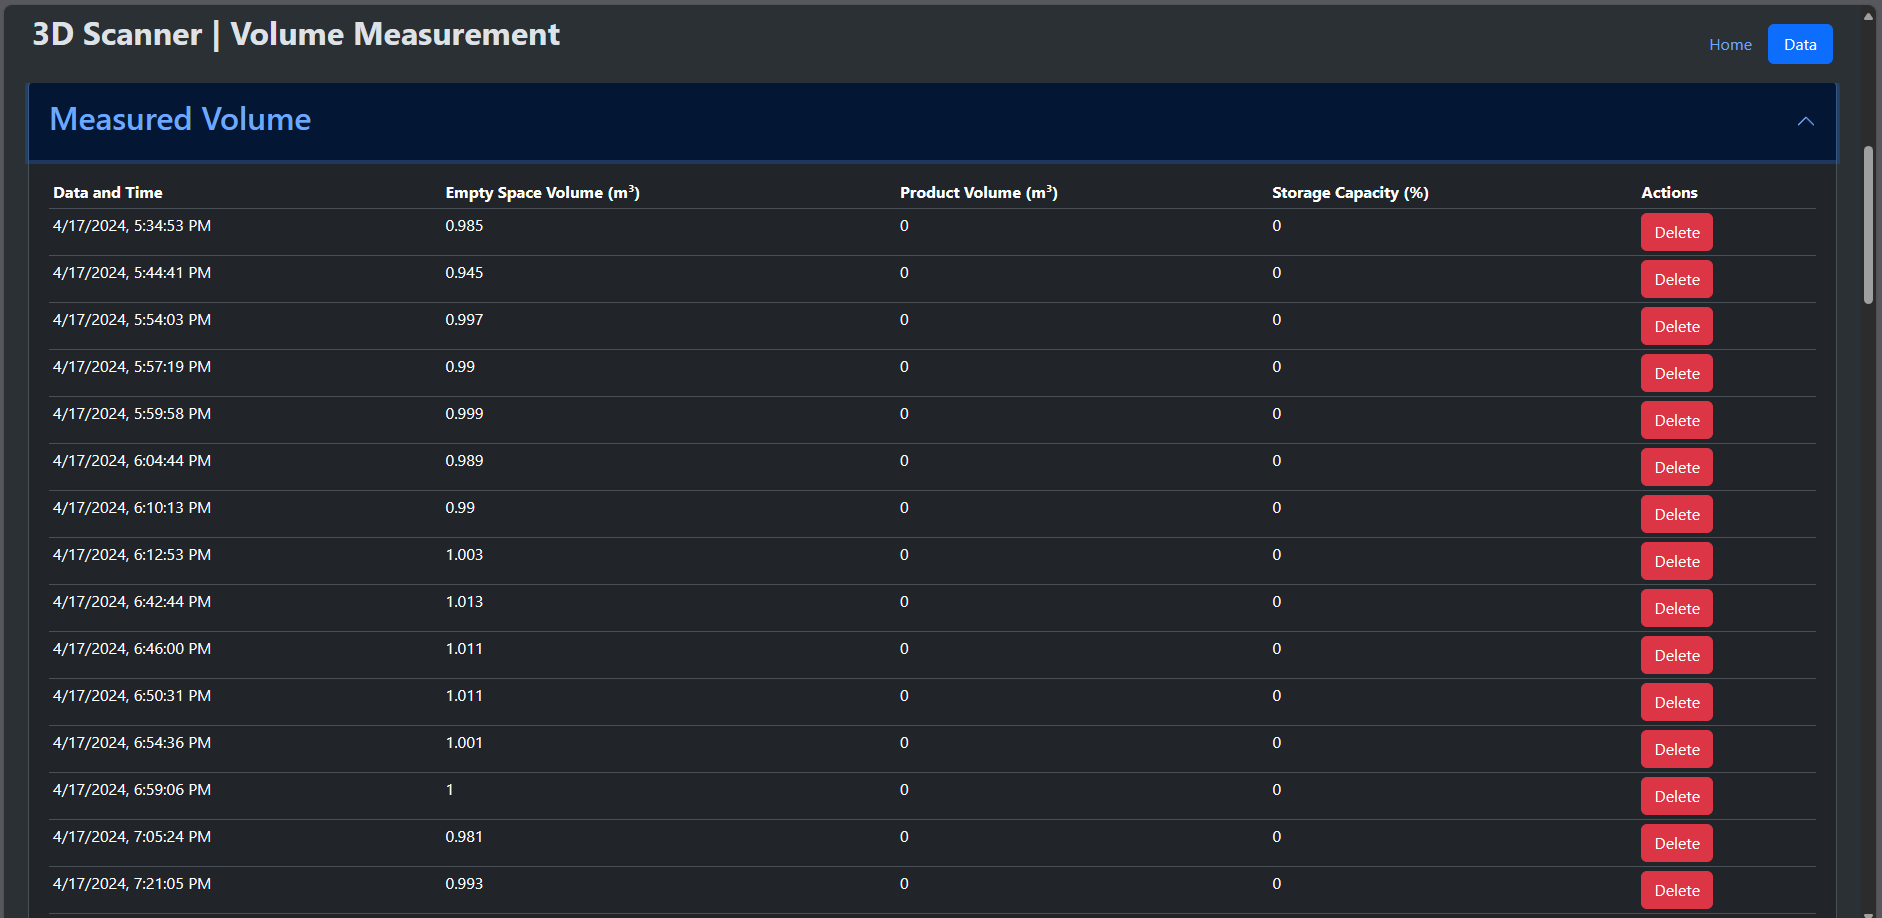
\includegraphics[width=0.9\textwidth]{Figures/main-dashboard-1}
	\caption{Data Dashboard Section Table}
	\label{ch4:fig:main-dashboard-1}
\end{figure}

\begin{figure}[H]
	\centering
	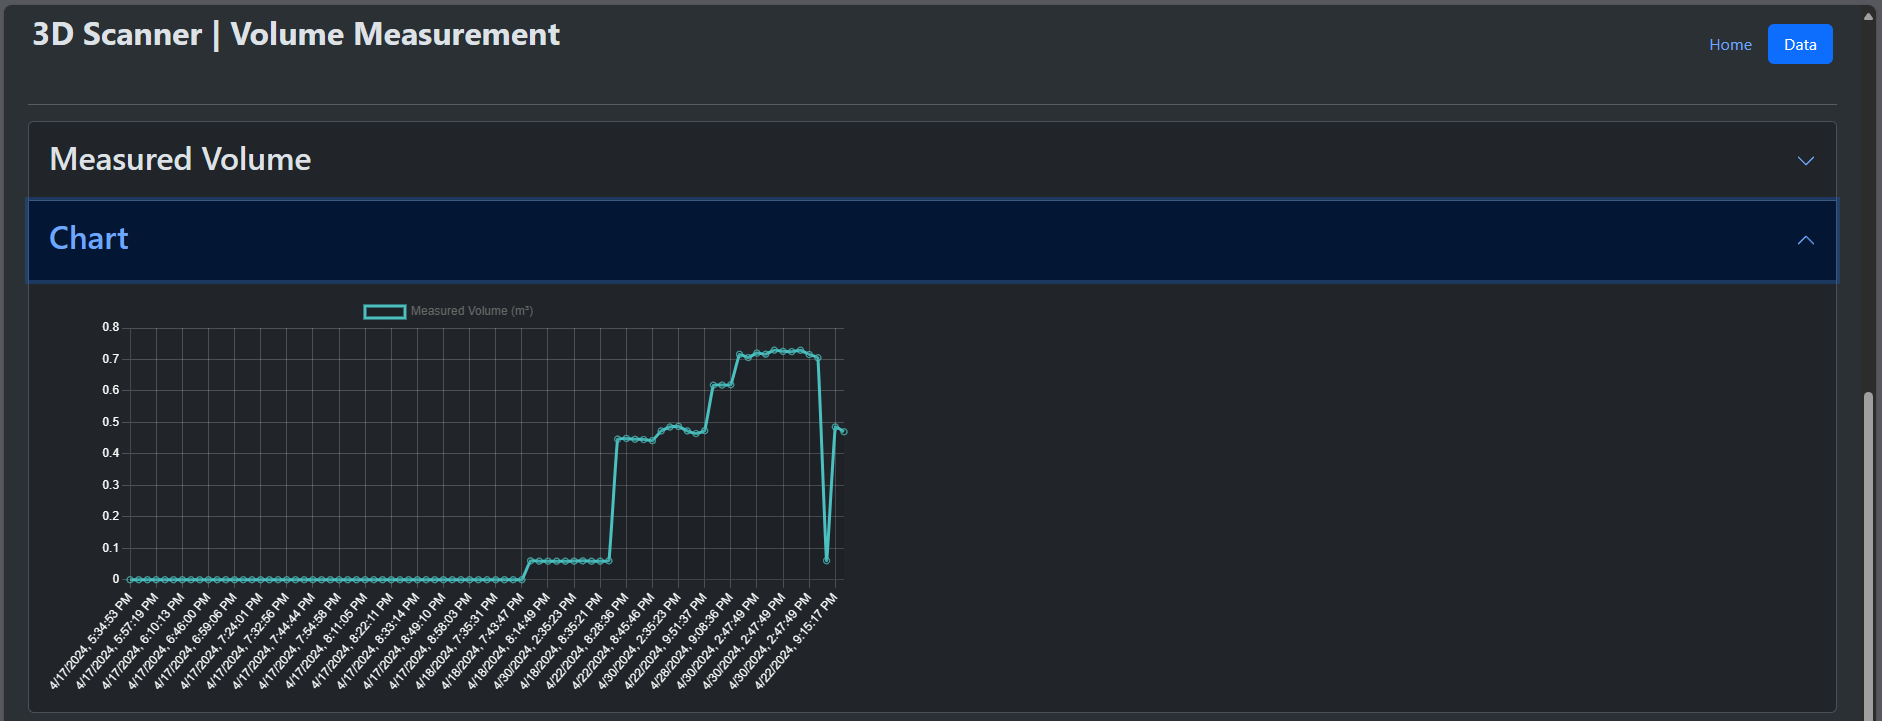
\includegraphics[width=0.9\textwidth]{Figures/main-dashboard-2}
	\caption{Data Dashboard Section Graph}
	\label{ch4:fig:main-dashboard-2}
\end{figure}

\section{Overall System Integration}
The 3D-PCSS and the Web interface were integrated and test their functionalities. This integration includes verifying the connection between the system and the web interface. After verifying the connection between the systems, further tests were conducted to ensure successfully interaction and functionality between the two components. This integration process aimed to validate the overall system's capability to communicate effectively,perform intended tasks such as send and receive command, and visualizing data.


\section{Testing Result and Data Analysis}

After conducting the various tests outlined in Section \ref{ch3:sec:TestingAndEvaluation}, the performance and accuracy of the overall system were evaluated. This section presents the results of each test case along with analysis of the data collected.

\subsection{Created Mock-up Storage Bin}
The design specifications outlined of the proposed storage bin in section \ref{ch3:subsec:constructing-of-storage-bin} were implemented to construct a mock-up storage bin. In the actual mock-up bin consists of three distinct geometric shapes as depicted in Figure \ref{ch4:fig:constructed-storage-bin}. The dimensions of each shape were manually measured using a steel tape measure.

The rectangular shape of the bin measures 2.775 meters in height, with lengths and widths of 0.5 and 0.69 meters respectively. The pyramidal frustum shape has an upper length and width of 0.5 and 0.69 meters respectively, with a height of 0.03 meters, and a lower length and width of 0.42 meters. Lastly, the conical frustum shape features a top radius of 0.21 meters, a bottom radius of 0.17 meters, and a height of 0.42 meters.

With these dimensions, the individual and total volume capacities of the storage bin were calculated. Table \ref{ch4:tab:volume-calculation} provides a summary of the measured individual and total volume capacity of the bin. \\


\begin{table}[H]
	\centering
	\caption{Individual and Total Volume of the Storage Bin}
	\label{ch4:tab:volume-calculation}
	\begin{tabular}{l r}
		\toprule
		\textbf{Shape}    & \textbf{Actual Volume ($m^{3}$)} \\ \midrule

		Rectangular       & 0.9573                           \\

		Pyramidal Frustum & 0.0077                           \\

		Conical Frustum   & 0.0478088                        \\ \midrule

		Total             & 1.012875                         \\ \bottomrule
	\end{tabular}
\end{table}

\begin{figure}[H]
	\centering
	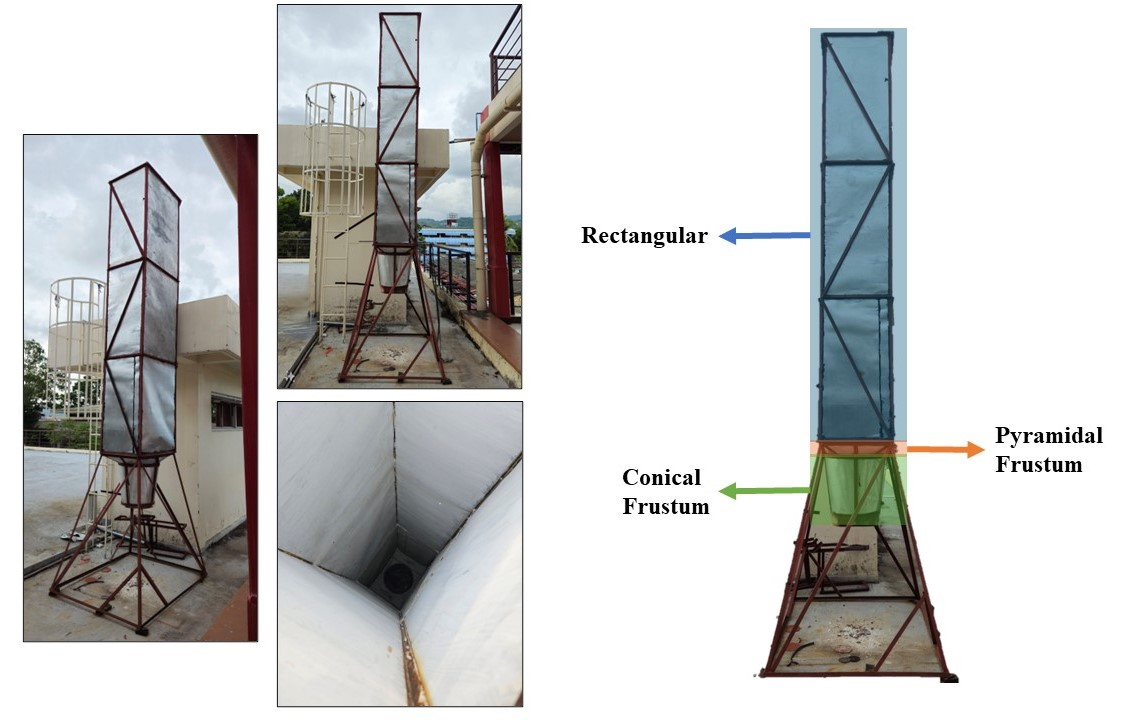
\includegraphics[width=0.9\textwidth]{Figures/constructed_storage_bin.jpg}
	\caption{Constructed Storage Bin Setup}
	\label{ch4:fig:constructed-storage-bin}
\end{figure}

\subsection{Actual System Setup}
The actual field system setup shown in figure \ref{ch4:fig:actual-system-setup} demonstrate the placement of the 3D-PCSS and the laptop where the user interface is running. The actual field of testing situated within the university premises.

\begin{figure}[H]
	\centering
	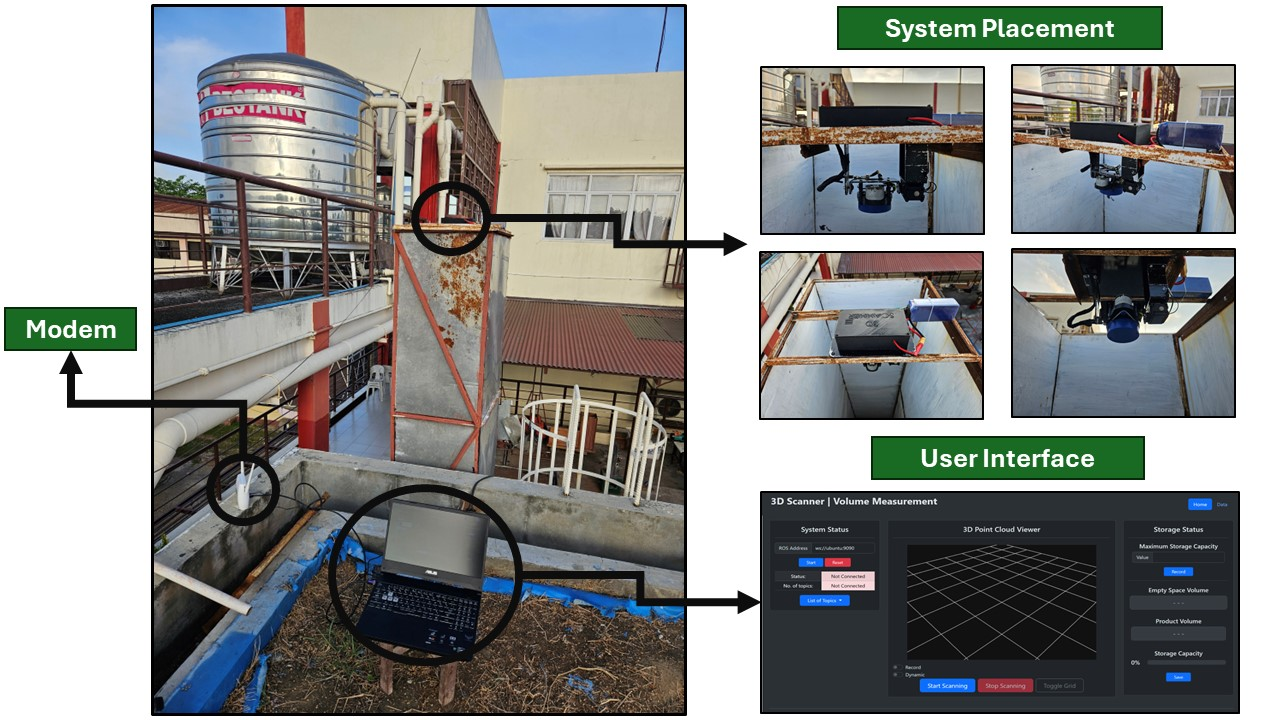
\includegraphics[width=1\textwidth]{Figures/actual-system-setup}
	\caption{Testing Field Actual System Setup}
	\label{ch4:fig:actual-system-setup}
\end{figure}


\subsection{Test Case 1: Empty Storage Bin Scanning}

Multiple scans of an empty storage bin were performed to evaluate the system's performance in accurately measuring the volume of the empty storage bin. Figure \ref{ch4:fig:empty-bin-point-cloud} shows the empty bin with the actual scanned point cloud shape. Table \ref{table:test_case_1_results} summarizes the results obtained from 37 scanning trials.

\begin{figure}[H]
	\centering
	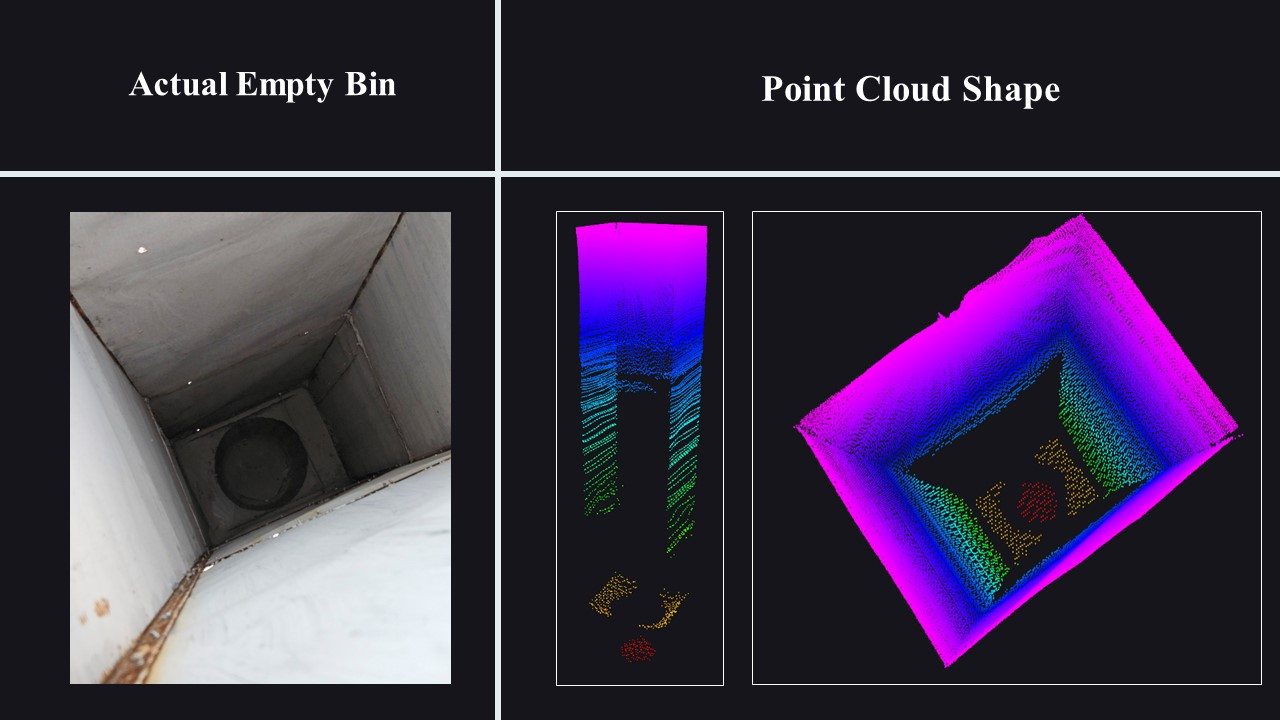
\includegraphics[width=1\textwidth]{Figures/empty-bin-point-cloud}
	\caption{Constructed Storage Bin Setup}
	\label{ch4:fig:empty-bin-point-cloud}
\end{figure}

\begin{table}[H]
	\centering
	\caption{Results of Test Case 1: Empty Storage Bin Scanning}
	\label{table:test_case_1_results}
	\begin{tabular}{l c r}
		\toprule
		\textbf{Trials} & \textbf{Actual Volume ($m^{3}$)} & \textbf{Measured Volume} ($m^{3}$) \\ \midrule

		1               & 1.012875                         & 0.997                              \\
		2               & 1.012875                         & 0.99                               \\
		3               & 1.012875                         & 0.999                              \\
		4               & 1.012875                         & 0.99                               \\
		5               & 1.012875                         & 1.003                              \\
		6               & 1.012875                         & 1.013                              \\
		7               & 1.012875                         & 1.011                              \\
		8               & 1.012875                         & 1.011                              \\
		9               & 1.012875                         & 1.001                              \\
		10              & 1.012875                         & 1                                  \\
		11              & 1.012875                         & 0.993                              \\
		12              & 1.012875                         & 1.007                              \\
		13              & 1.012875                         & 1.011                              \\
		14              & 1.012875                         & 1.019                              \\
		15              & 1.012875                         & 1.021                              \\
		16              & 1.012875                         & 1.013                              \\
		17              & 1.012875                         & 1.014                              \\
		18              & 1.012875                         & 1.006                              \\
		19              & 1.012875                         & 1.003                              \\
		20              & 1.012875                         & 1.01                               \\
		21              & 1.012875                         & 1.013                              \\
		22              & 1.012875                         & 1.016                              \\
		23              & 1.012875                         & 1.014                              \\
		24              & 1.012875                         & 1.014                              \\
		25              & 1.012875                         & 1.016                              \\
		26              & 1.012875                         & 1.015                              \\
		27              & 1.012875                         & 1.011                              \\
		28              & 1.012875                         & 1.011                              \\
		29              & 1.012875                         & 1.007                              \\
		30              & 1.012875                         & 1.016                              \\
		31              & 1.012875                         & 1.017                              \\
		32              & 1.012875                         & 1.009                              \\
		33              & 1.012875                         & 1.007                              \\
		34              & 1.012875                         & 1.017                              \\
		35              & 1.012875                         & 1.017                              \\
		36              & 1.012875                         & 1.014                              \\
		37              & 1.012875                         & 1.014                              \\ \bottomrule
	\end{tabular}
\end{table}

\begin{figure}[H]
	\centering
	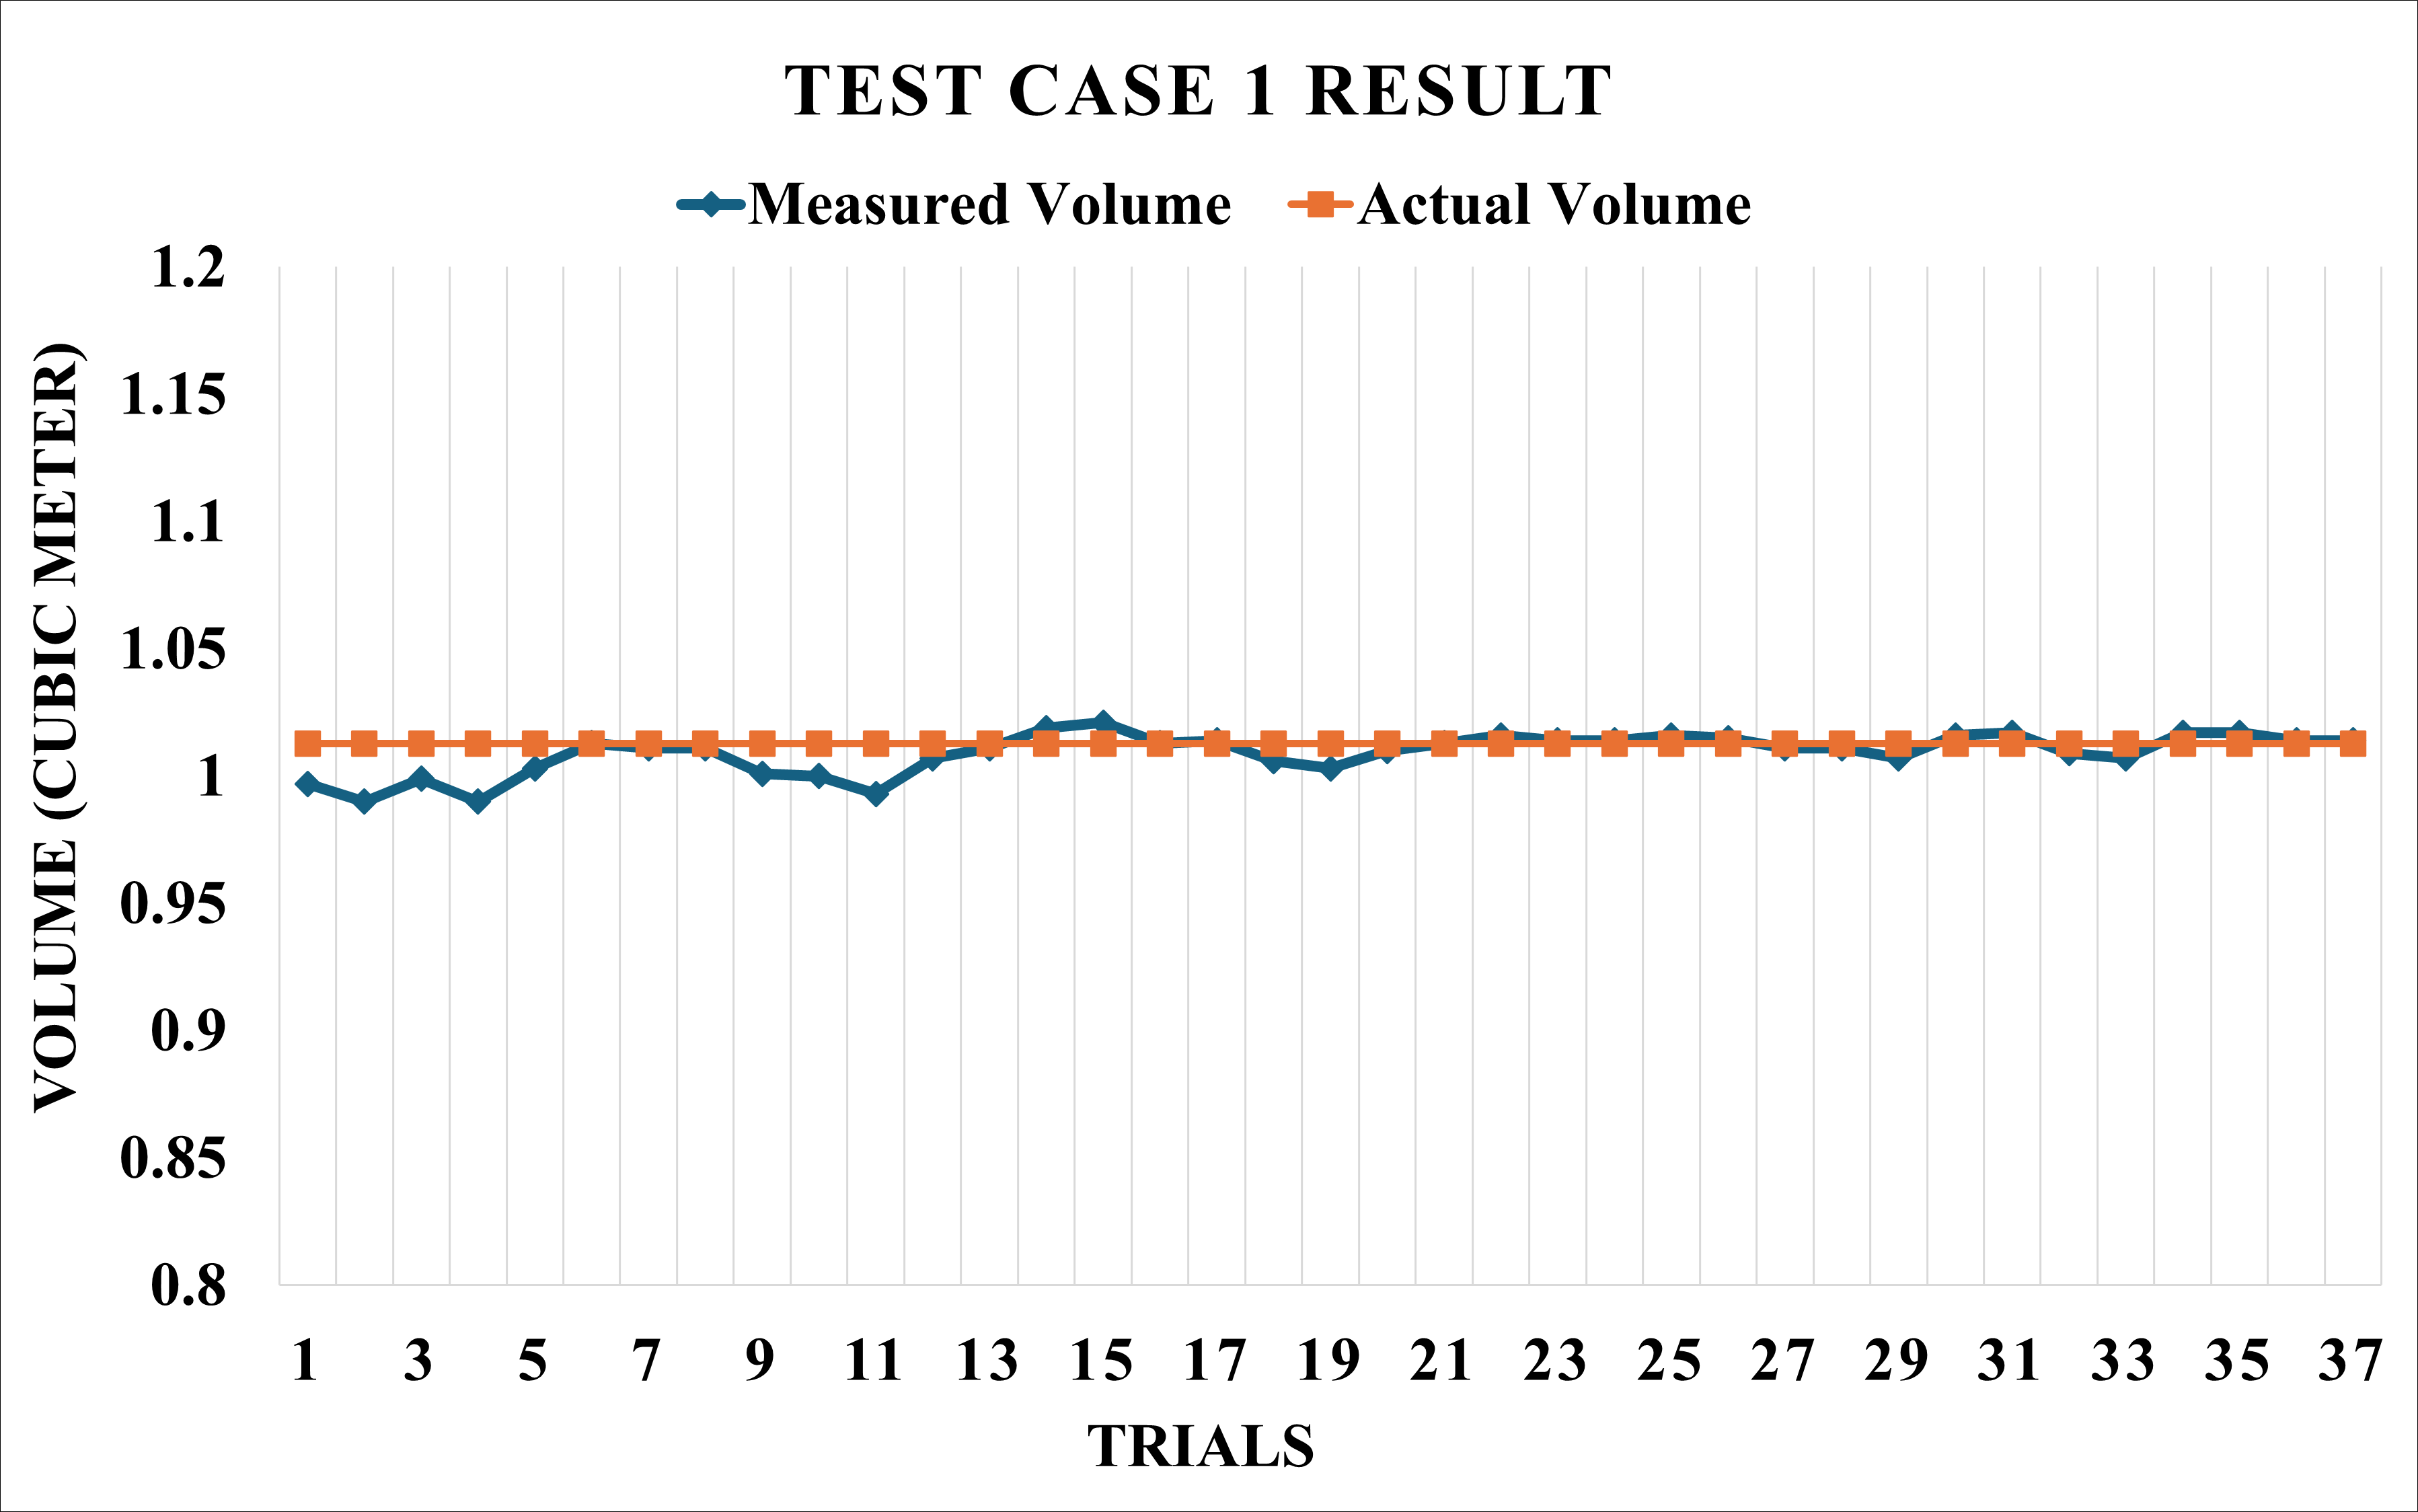
\includegraphics[width=0.8\textwidth]{Figures/test-case-1-graph}
	\caption{Distribution of the Measured Volume with 37 Trials on Test Case 1}
	\label{ch4:fig:test-case-1-graph}
\end{figure}

The average measured volume across all trials was determined to be 1.00919 $\pm$ 0.00784 $m^{3}$, indicating a standard deviation of 0.00784 $m^{3}$. With a gathered Mean Absolute Percentage Error (MAPE) of 0.599377608 \%. This average volume of the empty storage bin was subsequently used as the maximum volume capacity for the next testing cases. The distribution of the data gathered can be visualize in the figure \ref{ch4:fig:test-case-1-graph}

\subsection{Test Case 2: Filling the Storage Bin with Known Volume}

In this test case, three different scenarios were conducted to evaluate the system's accuracy in measuring the volume of flour filled into the storage bin with different storage percentage capacity such as: 5.8\%, 47.2\% and 70.3\% of the storage's maximum capacity, the storage bin was filled with a known volume using the container shown in figure \ref{ch4:fig:known-volume}. Each scenario conducted two different flour surface contour as outline in section \ref{ch3:subsec:test-case-2}. The results show the different flour surface contour first, followed by the data table.

\begin{figure}[H]
	\centering
	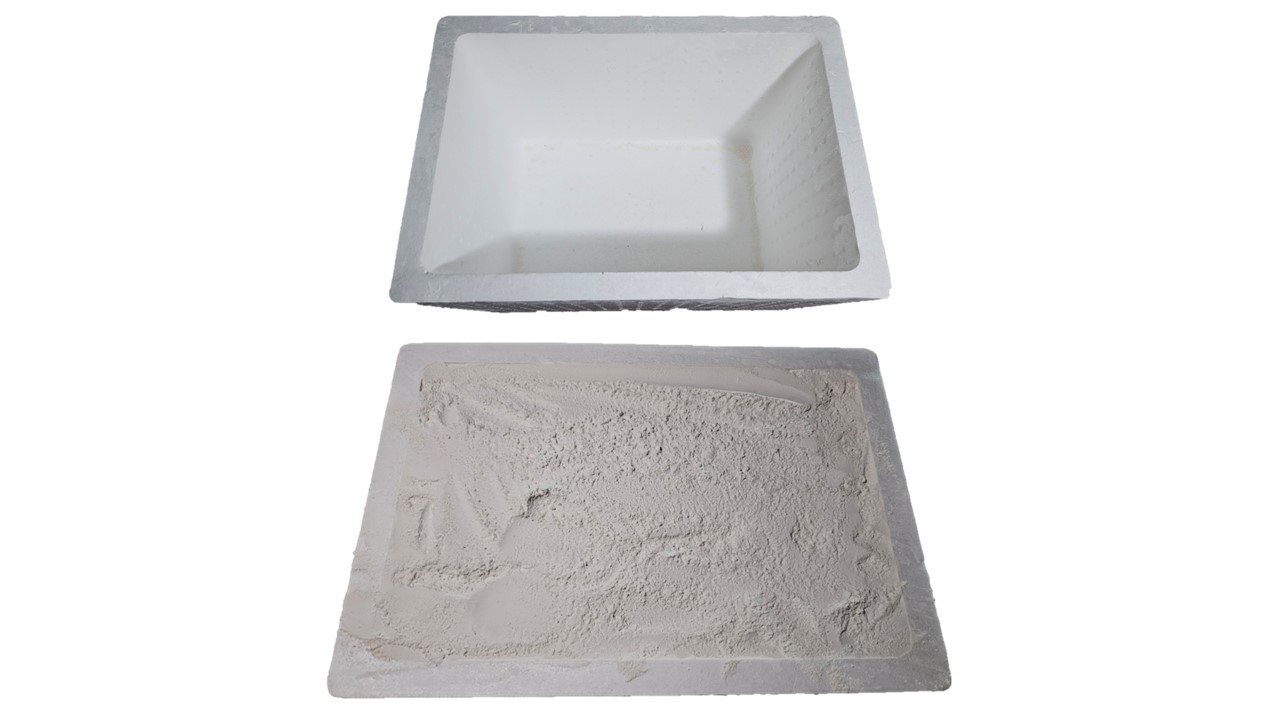
\includegraphics[width=0.8\textwidth]{Figures/known-volume}
	\caption{Container with a Known Volume Used for Testing}
	\label{ch4:fig:known-volume}
\end{figure}


\subsubsection*{Test Case 2.1: Storage Bin Filled to 5.8\% of Maximum Capacity}

\begin{figure}[H]
	\centering
	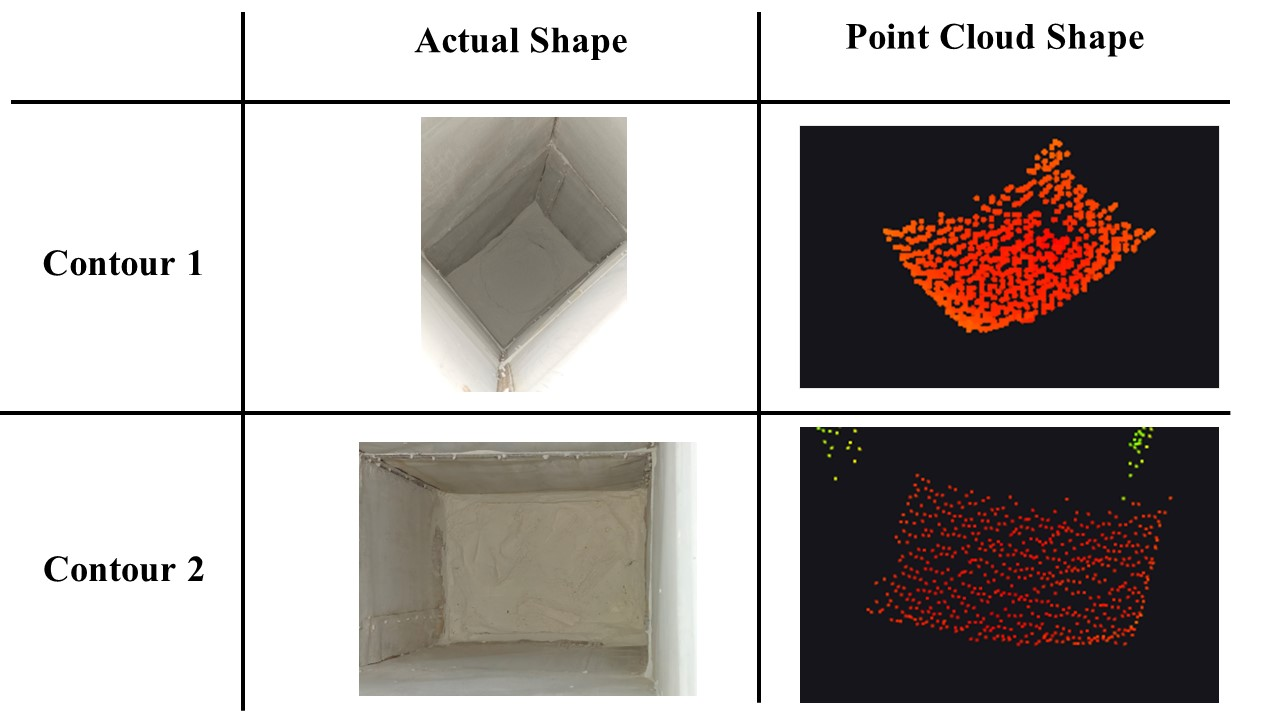
\includegraphics[width=0.8\textwidth]{Figures/test_2-1_contours}
	\caption{Different Flour Surface Contour of Test 2.1}
	\label{ch4:fig:test_2-1_contours}
\end{figure}

\begin{table}[H]
	\centering
	\caption{Test Case 2.1 Result}
	\label{table:test_case_2-1_results}
	\begin{tabular}{l c c r}
		\toprule
		\textbf{Trials} & \multicolumn{2}{c}{\textbf{Measured Volume ($m^{3}$)}} & \textbf{Actual Volume} ($m^{3}$)          \\
		{}              & Contour 1                                              & Contour 2                        & {}     \\ \midrule
		1               & 0.06                                                   & 0.0592                           & 0.0594 \\
		2               & 0.05934                                                & 0.0601                           & 0.0594 \\
		3               & 0.058943                                               & 0.0589                           & 0.0594 \\
		4               & 0.05976                                                & 0.0591                           & 0.0594 \\
		5               & 0.059678                                               & 0.0602                           & 0.0594 \\ \midrule
		Average         & 0.059678                                               & 0.0595                           & {}     \\ \bottomrule
	\end{tabular}
\end{table}

\begin{figure}[H]
	\centering
	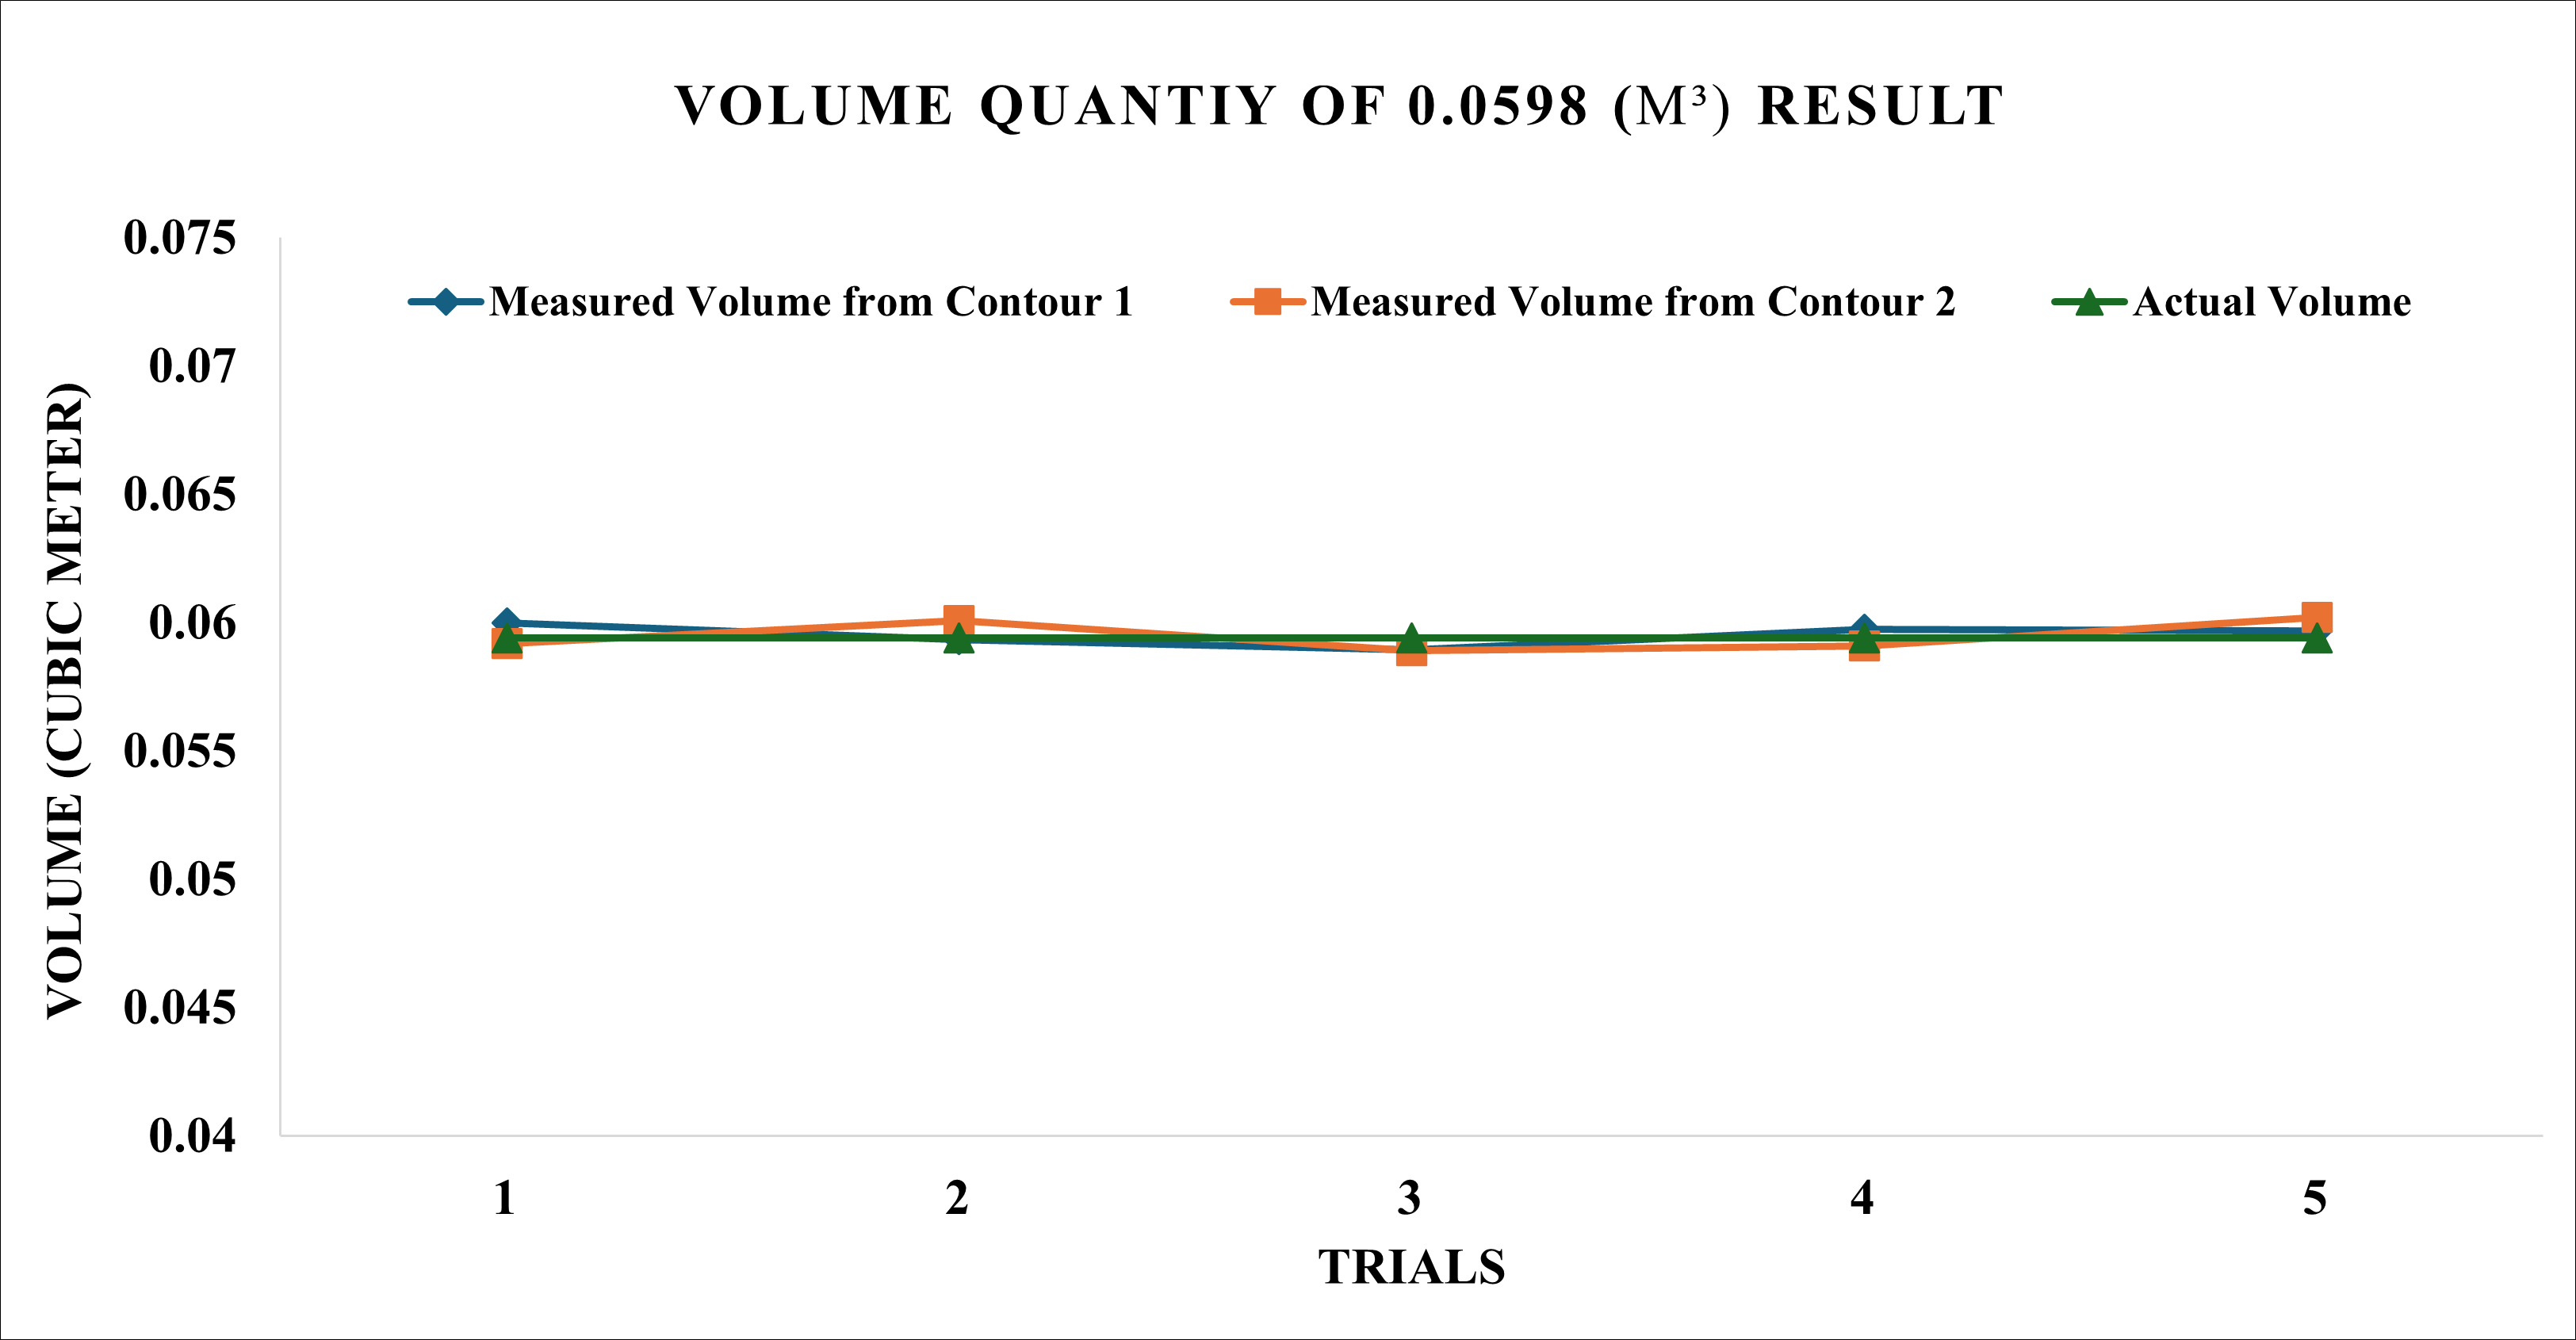
\includegraphics[width=0.8\textwidth]{Figures/test-case-2-1-graph}
	\caption{Distribution of the Measured Volume on Test Case 2.1}
	\label{ch4:fig:test-case-2-1-graph}
\end{figure}



The results from Test Case 2.1 gathered an average measured volume of 0.059678 $m^{3}$ and 0.0595 $m^{3}$ and a deviation of 0.00036 $m^{3}$ and 0.00054 $m^{3}$ from contour 1 and 2 respectively. Contour 1 achieved a MAPE of 0.591\%, while the contour 2 have a MAPE of 0.8417\%. Overall, Test Case 2.1 gathered an average measured volume with standard deviation of 0.0595221 $\pm$ 0.0004626 $m^{3}$ and a MAPE of 0.7163\%.

%\subsection{Discussion}

%%%The test results demonstrate the effectiveness and accuracy of the developed 3D-PCSS in measuring the volume of both empty and filled storage bins. The system consistently provided reliable measurements across multiple trials and scenarios, validating its suitability for practical applications in various industries. Further analysis of the data collected revealed minor discrepancies between the measured and actual volumes, which can be attributed to factors such as sensor calibration and environmental conditions. Overall, the system performed satisfactorily and met the objectives set forth in this study. \\

%%%%%%%%%%%%%%%%%%%%%%%%%%%%%%%%%%%%%%%%%%%%%%

\subsubsection*{Test Case 2.2: Storage Bin Filled to 47.2\% of Maximum Capacity}

\begin{figure}[H]
	\centering
	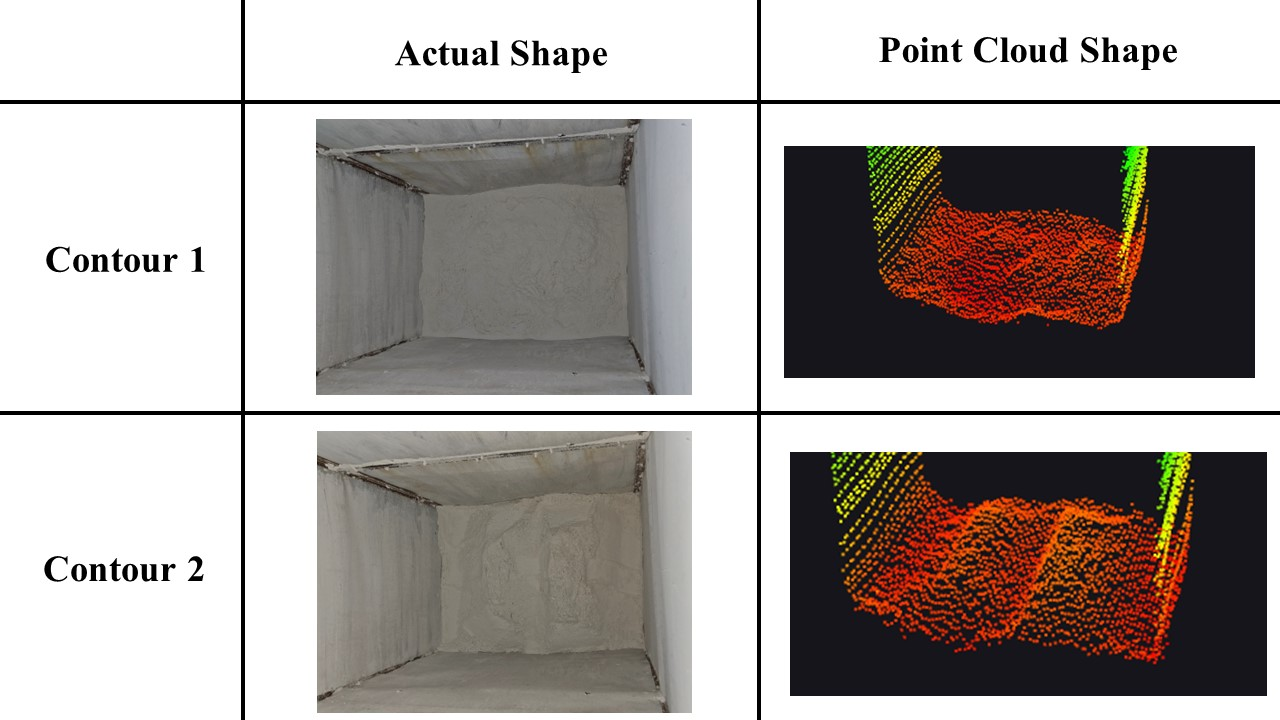
\includegraphics[width=0.8\textwidth]{Figures/test_2-2_contours}
	\caption{Different Flour Surface Contour of Test 2.2}
	\label{ch4:fig:test_2-2_contours}
\end{figure}
\begin{table}[H]
	\centering
	\caption{Test Case 2.2 Result}
	\label{table:test_case_2-2_results}
	\begin{tabular}{l c c r}
		\toprule
		\textbf{Trials} & \multicolumn{2}{c}{\textbf{Measured Volume ($m^{3}$)}} & \textbf{Actual Volume} ($m^{3}$)          \\
		{}              & Contour 1                                              & Contour 2                        & {}     \\ \midrule
		1               & 0.470418                                               & 0.472914                         & 0.4752 \\
		2               & 0.470279                                               & 0.464461                         & 0.4752 \\
		3               & 0.472061                                               & 0.473782                         & 0.4752 \\
		4               & 0.4805594                                              & 0.485587                         & 0.4752 \\
		5               & 0.4770345                                              & 0.470211                         & 0.4752 \\ \midrule
		Average         & 0.47407038                                             & 0.473391                         & {}     \\ \bottomrule
	\end{tabular}
\end{table}

\begin{figure}[H]
	\centering
	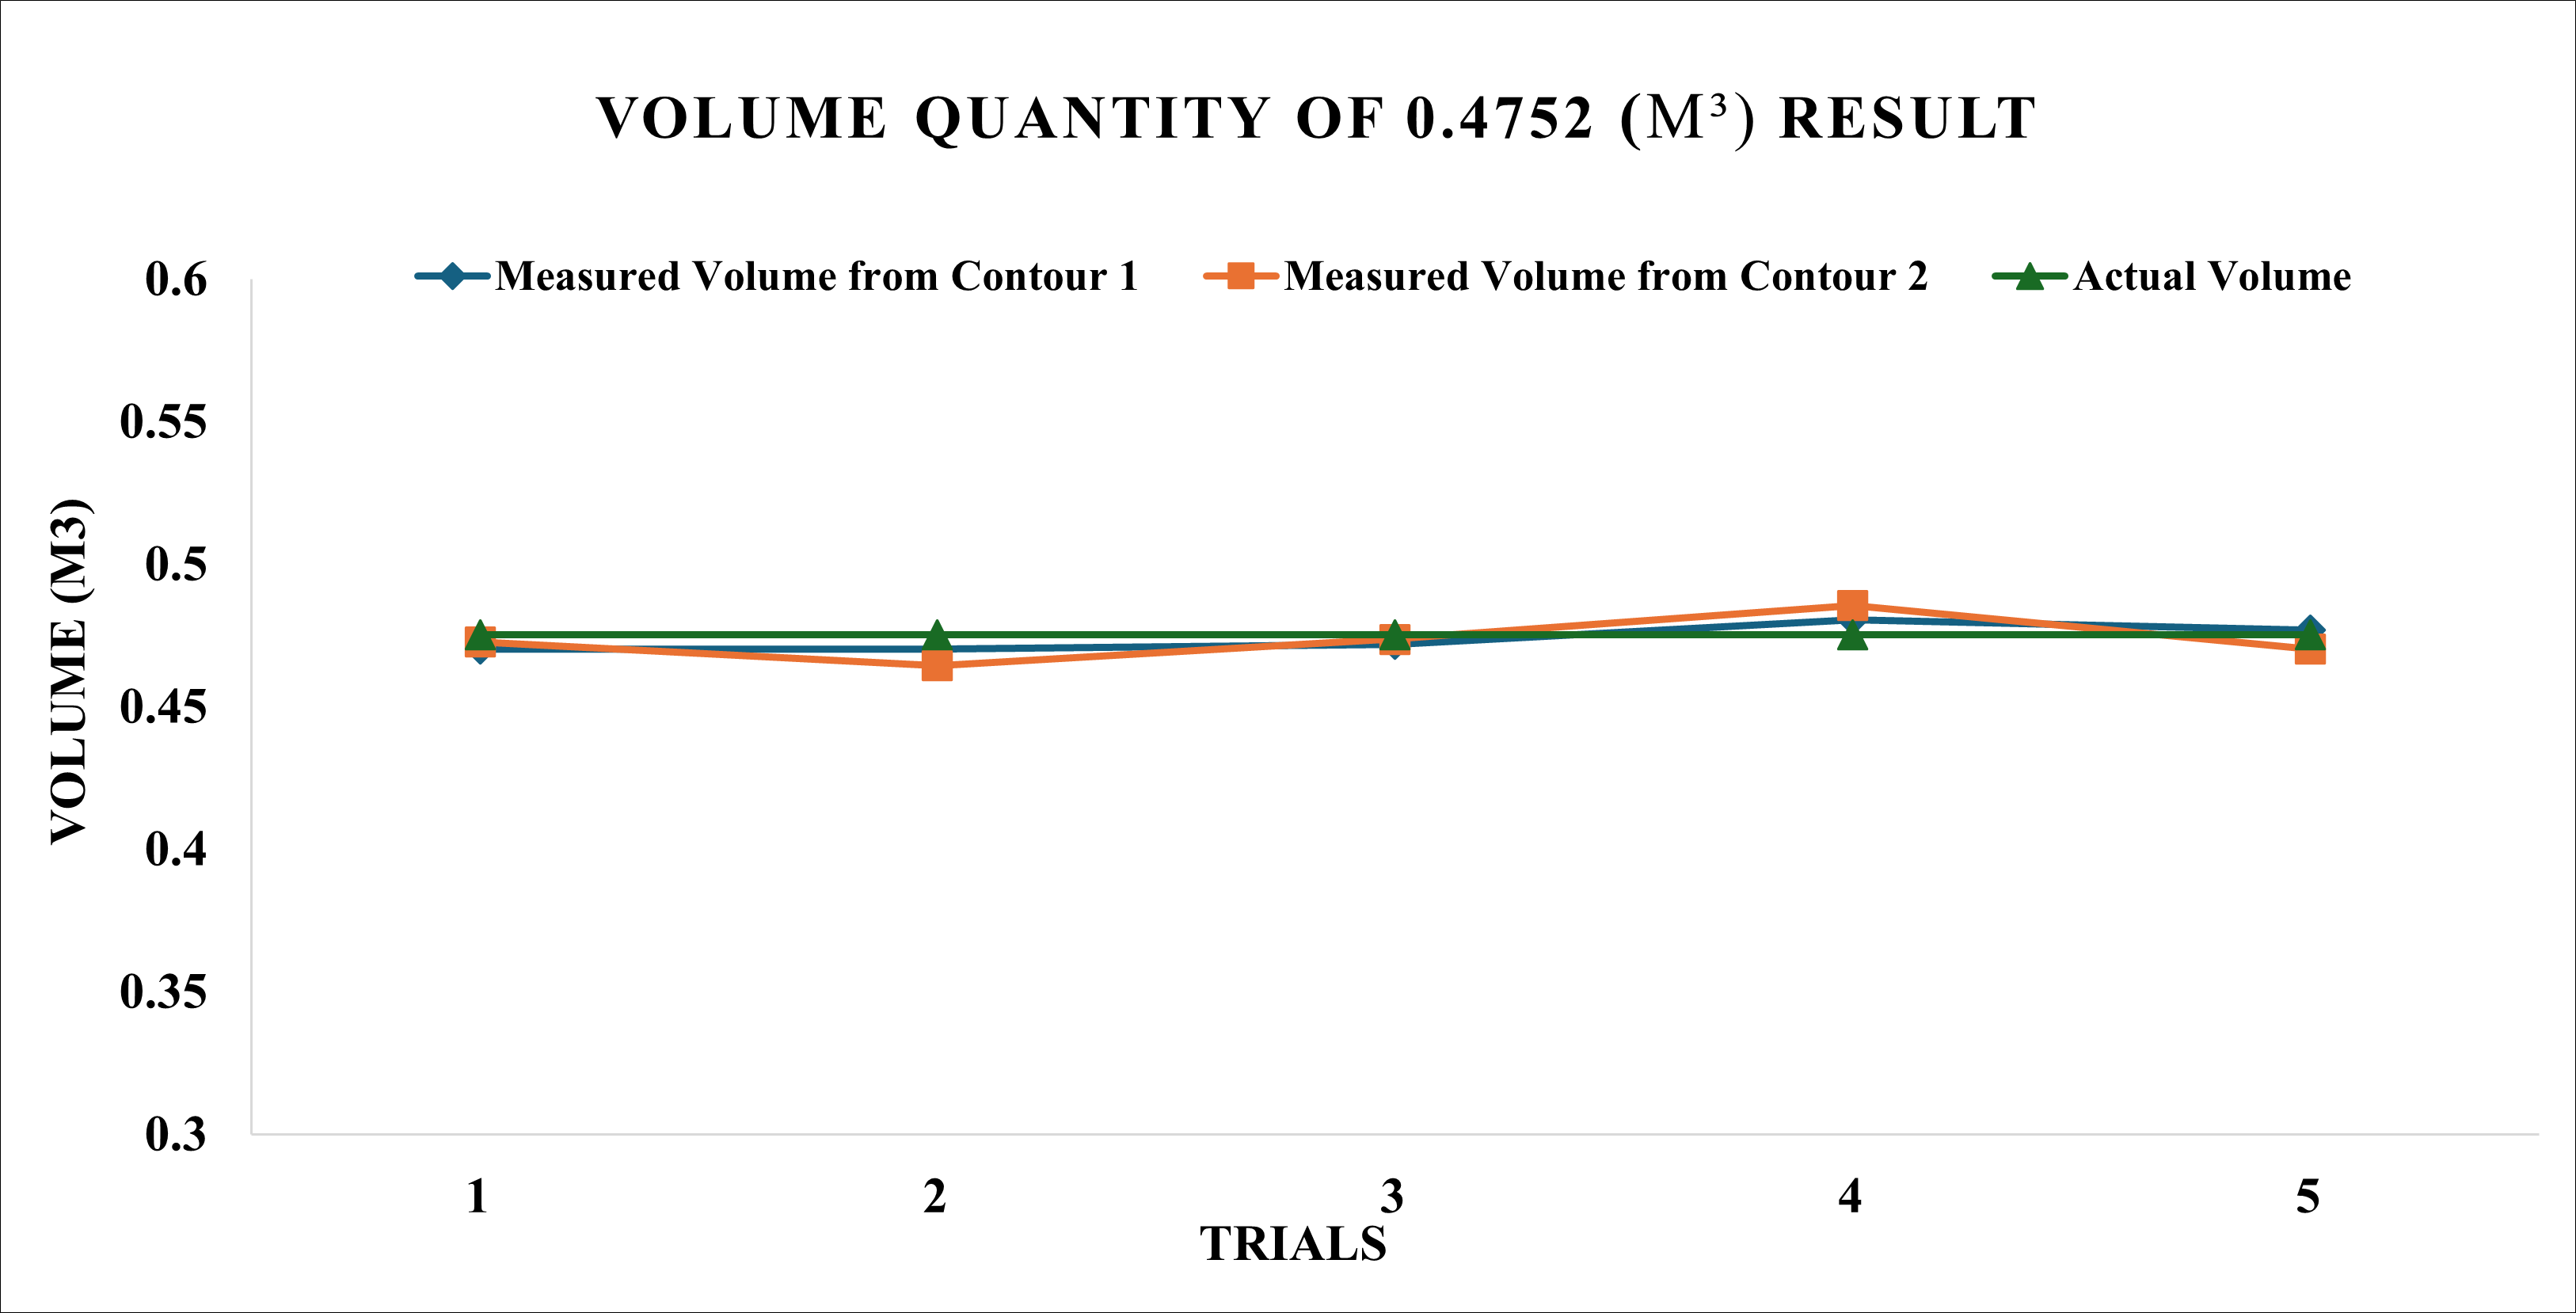
\includegraphics[width=0.8\textwidth]{Figures/test-case-2-2-graph}
	\caption{Distribution of the Measured Volume on Test Case 2.2}
	\label{ch4:fig:test-case-2-2-graph}
\end{figure}

The results from Test Case 2.2 gathered an average measured volume of 0.47407038 $m^{3}$ and 0.4733912158 $m^{3}$ and a deviation of 0.00406 $m^{3}$ and 0.00691 $m^{3}$ from contour 1 and 2 respectively. Contour 1 achieved a MAPE of 0.8432\%, while the contour 2 have a MAPE of 1.2549\%. Overall, Test Case 2.2 gathered an average measured volume with a standard deviation of 0.47373 $\pm$ 0.00568 $m^{3}$ and a MAPE of 1.04912\%.

\subsubsection*{Test Case 2.3: Storage Bin Filled to 70.37\% of Maximum Capacity}
\begin{figure}[H]
	\centering
	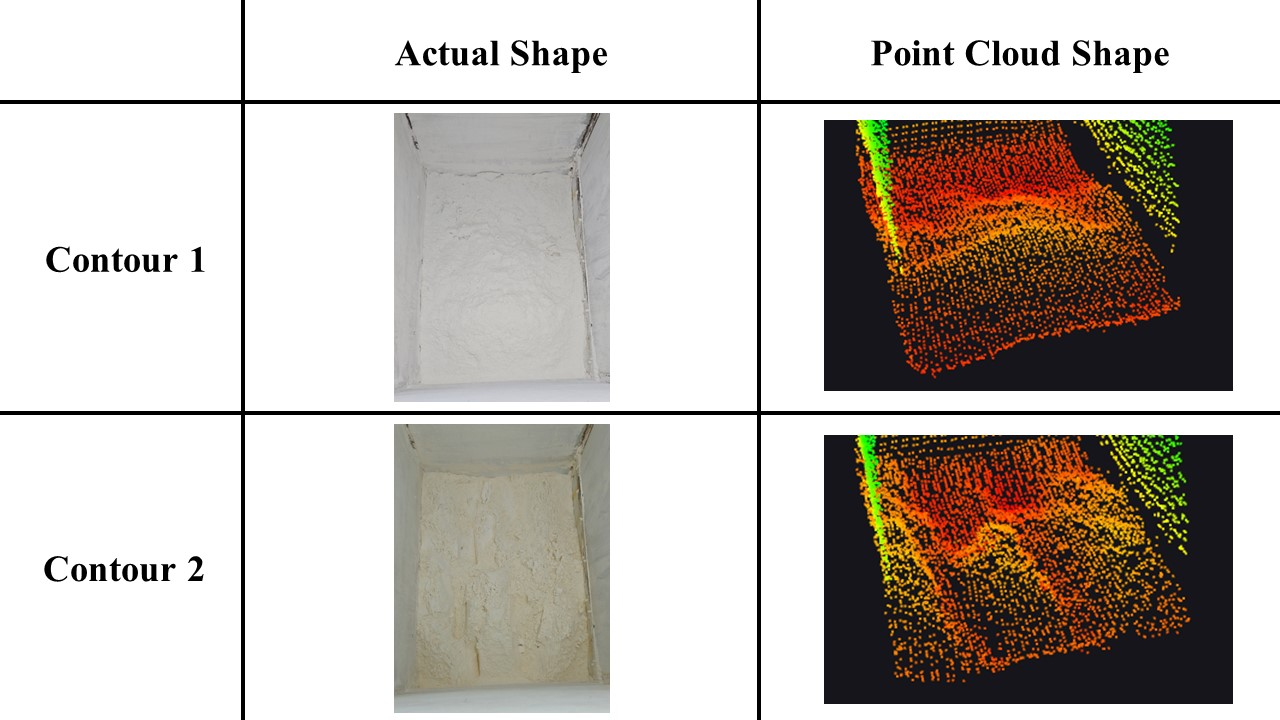
\includegraphics[width=0.8\textwidth]{Figures/test_2-3_contours}
	\caption{Different Flour Surface Contour of Test 2.3}
	\label{ch4:fig:test_2-3_contours}
\end{figure}

\begin{table}[H]
	\centering
	\caption{Test Case 2.3 Result}
	\label{table:test_case_2-3_results}
	\begin{tabular}{l c c r}
		\toprule
		\textbf{Trials} & \multicolumn{2}{c}{\textbf{Measured Volume ($m^{3}$)}} & \textbf{Actual Volume} ($m^{3}$)          \\
		{}              & Contour 1                                              & Contour 2                        & {}     \\ \midrule
		1               & 0.716327                                               & 0.725803                         & 0.7128 \\
		2               & 0.706001                                               & 0.724873                         & 0.7128 \\
		3               & 0.720251                                               & 0.729404                         & 0.7128 \\
		4               & 0.71687                                                & 0.715844                         & 0.7128 \\
		5               & 0.729654                                               & 0.705429                         & 0.7128 \\ \midrule
		Average         & 0.7178206                                              & 0.7202706                        & {}     \\ \bottomrule
	\end{tabular}
\end{table}

\begin{figure}[H]
	\centering
	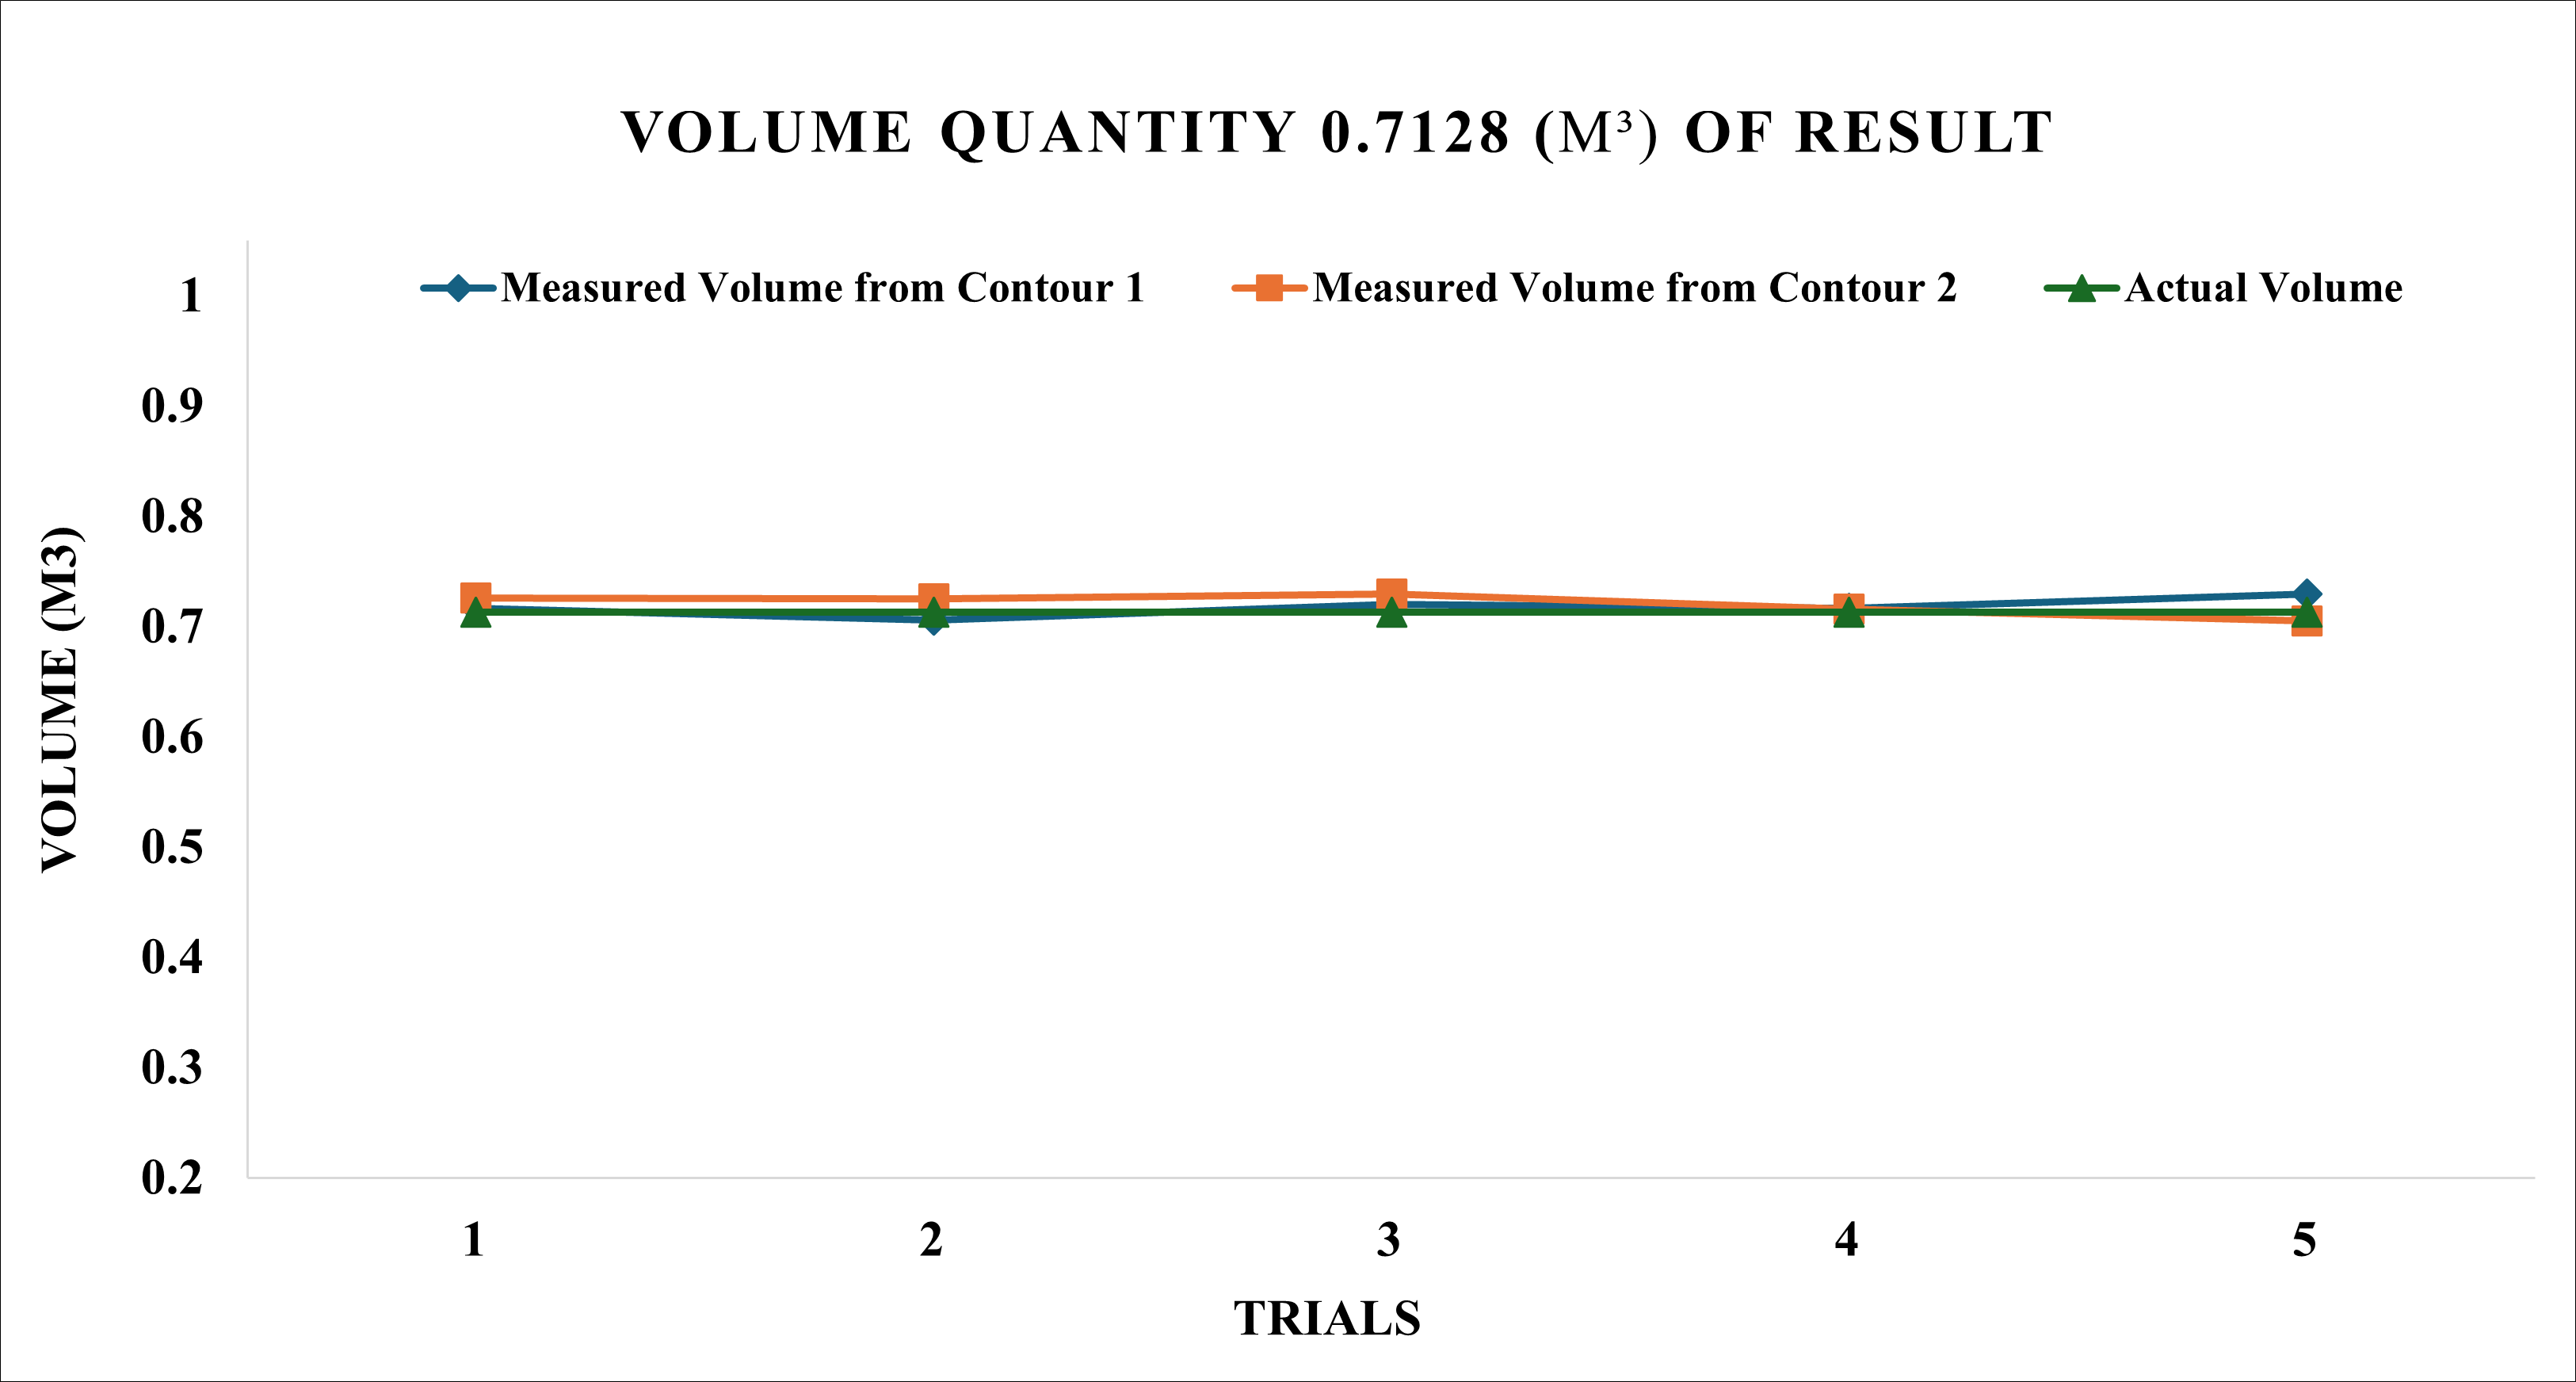
\includegraphics[width=0.8\textwidth]{Figures/test-case-2-3-graph}
	\caption{Distribution of the Measured Volume on Test Case 2.3}
	\label{ch4:fig:test-case-2-3-graph}
\end{figure}


The results from Test Case 2.3 gathered an average measured volume of 0.7178206 $m^{3}$ and 0.7202706 $m^{3}$ and a deviation of 0.0076 $m^{3}$ and 0.0086 $m^{3}$ from contour 1 and 2 respectively. Contour 1 achieved a MAPE of 1.08588\%, while the contour 2 have a MAPE of 1.4617\%. Overall, Test Case 2.3 gathered an average measured volume with a standard deviation of 0.719 $\pm$ 0.008239 $m^{3}$ and a MAPE of 1.27379\%.

\subsubsection*{Summary of Test Case 2 Result}
\begin{table}[H]
	\centering
	\caption{Summary of the of Test Case 2}
	\label{ch4:tab:test-2-summary}
	\begin{tabular}{l c r}
		\toprule
		\textbf{Test} & \textbf{Average Measured Volume with Deviation ($m^{3}$)} & \textbf{MAPE (\%)} \\ \midrule

		2.1           & 0.0595 $\pm$ 0.0004626                                    & 0.71633            \\

		2.2           & 0.47373 $\pm$ 0.00568                                     & 1.04912            \\

		2.3           & 0.719 $\pm$ 0.00824                                       & 1.27379            \\ \midrule

		Average       & {}                                                        & 1.01308            \\ \bottomrule
	\end{tabular}
\end{table}

The table \ref{ch4:tab:test-2-summary} indicates that the system achieved an average MAPE of 1.01308 across the three conducted tests. This suggests that the system is capable of accurately measuring the volume of the flour product across varying storage capacities, up to a maximum level of 70.3\%.

\subsection{Summary of the Conducted Test Cases}

\begin{table}[H]
	\centering
	\caption{Summary of the of Test Case 2}
	\label{ch4:tab:test-cases-summary}
	\begin{tabular}{l l c r}
		\toprule
		\multicolumn{2}{l}{\textbf{Test Cases}} & \textbf{Average Measured Volume with Deviation ($m^{3}$)} & \textbf{MAPE (\%)}                \\ \midrule

		\multicolumn{2}{l}{1}                   & 1.009189 $\pm$ 0.0078356                                  & 0.5993776                         \\

		{}                                      & 2.1                                                       & 0.0595 $\pm$ 0.0004626 & 0.71633  \\

		2                                       & 2.2                                                       & 0.47373 $\pm$ 0.00568  & 1.04912  \\

		{}                                      & 2.3                                                       & 0.719 $\pm$ 0.00824    & 1.27379  \\ \midrule

		Average                                 & {}                                                        & {}                     & 0.909655 \\ \bottomrule
	\end{tabular}
\end{table}

The table \ref{ch4:tab:test-cases-summary} summarizes the two test cases conducted. The system achieved an average MAPE of 0.909655\% indicates an error of $<1\%$ with a highest error of 1.27379\% and lowest error of 0.5993776\%.